% Kurt: things to do:
%1) fix Table XII about SVMs, we should not distinguish \sigma vs. not \sigma. If we can have only with sigma, great. DONE.
%2) Discrete features for Financial? DONE.
%3) Decide what to do with the extra space: a) add Figure 1, the ``big picture''. or b) take it out and make more tables 2-column?
%4) some of the references came out crazy, e.g. 6 lists a URL, not necessary. CURRENTLY 9 PAGES. Again, please remove URLs, don't say ``londong, UK''. You can move this info into the ``comment field.''

%5) Can we get the tables to appear earlier?
%% bare_conf.tex
%% V1.3
%% 2007/01/11
%% by Michael Shell
%% See:
%% http://www.michaelshell.org/
%% for current contact information.
%%
%% This is a skeleton file demonstrating the use of IEEEtran.cls
%% (requires IEEEtran.cls version 1.7 or later) with an IEEE conference paper.
%%
%% Support sites:
%% http://www.michaelshell.org/tex/ieeetran/
%% http://www.ctan.org/tex-archive/macros/latex/contrib/IEEEtran/
%% and
%% http://www.ieee.org/

%%*************************************************************************
%% Legal Notice:
%% This code is offered as-is without any warranty either expressed or
%% implied; without even the implied warranty of MERCHANTABILITY or
%% FITNESS FOR A PARTICULAR PURPOSE!
%% User assumes all risk.
%% In no event shall IEEE or any contributor to this code be liable for
%% any damages or losses, including, but not limited to, incidental,
%% consequential, or any other damages, resulting from the use or misuse
%% of any information contained here.
%%
%% All comments are the opinions of their respective authors and are not
%% necessarily endorsed by the IEEE.
%%
%% This work is distributed under the LaTeX Project Public License (LPPL)
%% ( http://www.latex-project.org/ ) version 1.3, and may be freely used,
%% distributed and modified. A copy of the LPPL, version 1.3, is included
%% in the base LaTeX documentation of all distributions of LaTeX released
%% 2003/12/01 or later.
%% Retain all contribution notices and credits.
%% ** Modified files should be clearly indicated as such, including  **
%% ** renaming them and changing author support contact information. **
%%
%% File list of work: IEEEtran.cls, IEEEtran_HOWTO.pdf, bare_adv.tex,
%%                    bare_conf.tex, bare_jrnl.tex, bare_jrnl_compsoc.tex
%%*************************************************************************

% *** Authors should verify (and, if needed, correct) their LaTeX system  ***
% *** with the testflow diagnostic prior to trusting their LaTeX platform ***
% *** with production work. IEEE's font choices can trigger bugs that do  ***
% *** not appear when using other class files.                            ***
% The testflow support page is at:
% http://www.michaelshell.org/tex/testflow/



% Note that the a4paper option is mainly intended so that authors in
% countries using A4 can easily print to A4 and see how their papers will
% look in print - the typesetting of the document will not typically be
% affected with changes in paper size (but the bottom and side margins will).
% Use the testflow package mentioned above to verify correct handling of
% both paper sizes by the user's LaTeX system.
%
% Also note that the "draftcls" or "draftclsnofoot", not "draft", option
% should be used if it is desired that the figures are to be displayed in
% draft mode.
%
\documentclass[conference]{IEEEtran}
% Add the compsoc option for Computer Society conferences.
%
% If IEEEtran.cls has not been installed into the LaTeX system files,
% manually specify the path to it like:
% \documentclass[conference]{../sty/IEEEtran}





% Some very useful LaTeX packages include:
% (uncomment the ones you want to load)


% *** MISC UTILITY PACKAGES ***
%
%\usepackage{ifpdf}
% Heiko Oberdiek's ifpdf.sty is very useful if you need conditional
% compilation based on whether the output is pdf or dvi.
% usage:
% \ifpdf
%   % pdf code
% \else
%   % dvi code
% \fi
% The latest version of ifpdf.sty can be obtained from:
% http://www.ctan.org/tex-archive/macros/latex/contrib/oberdiek/
% Also, note that IEEEtran.cls V1.7 and later provides a builtin
% \ifCLASSINFOpdf conditional that works the same way.
% When switching from latex to pdflatex and vice-versa, the compiler may
% have to be run twice to clear warning/error messages.






% *** CITATION PACKAGES ***
%
%\usepackage{cite}
% cite.sty was written by Donald Arseneau
% V1.6 and later of IEEEtran pre-defines the format of the cite.sty package
% \cite{} output to follow that of IEEE. Loading the cite package will
% result in citation numbers being automatically sorted and properly
% "compressed/ranged". e.g., [1], [9], [2], [7], [5], [6] without using
% cite.sty will become [1], [2], [5]--[7], [9] using cite.sty. cite.sty's
% \cite will automatically add leading space, if needed. Use cite.sty's
% noadjust option (cite.sty V3.8 and later) if you want to turn this off.
% cite.sty is already installed on most LaTeX systems. Be sure and use
% version 4.0 (2003-05-27) and later if using hyperref.sty. cite.sty does
% not currently provide for hyperlinked citations.
% The latest version can be obtained at:
% http://www.ctan.org/tex-archive/macros/latex/contrib/cite/
% The documentation is contained in the cite.sty file itself.






% *** GRAPHICS RELATED PACKAGES ***
%
\ifCLASSINFOpdf
\usepackage[pdftex]{graphicx}
  % declare the path(s) where your graphic files are
  % \graphicspath{{../pdf/}{../jpeg/}}
  % and their extensions so you won't have to specify these with
  % every instance of \includegraphics
  % \DeclareGraphicsExtensions{.pdf,.jpeg,.png}
\else
  % or other class option (dvipsone, dvipdf, if not using dvips). graphicx
  % will default to the driver specified in the system graphics.cfg if no
  % driver is specified.
\usepackage[dvips]{graphicx}
  % declare the path(s) where your graphic files are
  % \graphicspath{{../eps/}}
  % and their extensions so you won't have to specify these with
  % every instance of \includegraphics
  % \DeclareGraphicsExtensions{.eps}
\fi
% graphicx was written by David Carlisle and Sebastian Rahtz. It is
% required if you want graphics, photos, etc. graphicx.sty is already
% installed on most LaTeX systems. The latest version and documentation can
% be obtained at:
% http://www.ctan.org/tex-archive/macros/latex/required/graphics/
% Another good source of documentation is "Using Imported Graphics in
% LaTeX2e" by Keith Reckdahl which can be found as epslatex.ps or
% epslatex.pdf at: http://www.ctan.org/tex-archive/info/
%
% latex, and pdflatex in dvi mode, support graphics in encapsulated
% postscript (.eps) format. pdflatex in pdf mode supports graphics
% in .pdf, .jpeg, .png and .mps (metapost) formats. Users should ensure
% that all non-photo figures use a vector format (.eps, .pdf, .mps) and
% not a bitmapped formats (.jpeg, .png). IEEE frowns on bitmapped formats
% which can result in "jaggedy"/blurry rendering of lines and letters as
% well as large increases in file sizes.
%
% You can find documentation about the pdfTeX application at:
% http://www.tug.org/applications/pdftex





% *** MATH PACKAGES ***
%
\usepackage[cmex10]{amsmath}
% A popular package from the American Mathematical Society that provides
% many useful and powerful commands for dealing with mathematics. If using
% it, be sure to load this package with the cmex10 option to ensure that
% only type 1 fonts will utilized at all point sizes. Without this option,
% it is possible that some math symbols, particularly those within
% footnotes, will be rendered in bitmap form which will result in a
% document that can not be IEEE Xplore compliant!
%
% Also, note that the amsmath package sets \interdisplaylinepenalty to 10000
% thus preventing page breaks from occurring within multiline equations. Use:
%\interdisplaylinepenalty=2500
% after loading amsmath to restore such page breaks as IEEEtran.cls normally
% does. amsmath.sty is already installed on most LaTeX systems. The latest
% version and documentation can be obtained at:
% http://www.ctan.org/tex-archive/macros/latex/required/amslatex/math/

%Example for automatically rescaling equations. 
% This is very tricky.
%\begin{equation}
%\label{eq:pimax}
%\resizebox{.55\textwidth}{!}{$
%\begin{split}
%P(\jtable_{2}|\set{E},\ttable) \propto &
%P(\keys = [jack,101],\it{Gr} = A, \it{Sat} = 1|\it{Int} = \class, \it{Rank} = 1, \it{Rat} = 3, \it{Diff}=1)\\
%\times & P(\keys = [jack,102],\it{Gr} = B, \it{Sat} = 2|\it{Int} = \class, \it{Rank} = 1, \it{Rat} = 2, \it{Diff}=2).
%\end{split}$
%}
%\end{equation}

%\usepackage{times}
%\usepackage[normaltitle,normalbib,normalmargins,normalindent]{savetrees}
\usepackage{amsmath}
\usepackage{amsfonts}
\usepackage{amssymb}
\usepackage{graphicx}
\usepackage{url}
%\usepackage{subfigure}
\usepackage{epstopdf}
\setcounter{MaxMatrixCols}{30}
%\usepackage{algorithm}
%\usepackage{algorithmic}
\usepackage{subfigure}
%\usepackage{subcaption}
\usepackage{fancyhdr}
\graphicspath{{../}{figures/}}
\usepackage{todonotes}

\DeclareMathOperator*{\argmax}{argmax}
\DeclareMathOperator*{\argmin}{argmin}
%\DeclareMathOperator{\pattern}{\pi}
\DeclareMathOperator{\Poly}{\mathbf{\mathrm{P}}}
\DeclareMathOperator{\RP}{\mathbf{\mathrm{RP}}}
%\DeclareMathOperator{\FP}{\mathbf{\mathrm{FP}}}
\DeclareMathOperator{\NP}{\mathbf{\mathrm{NP}}}
%\DeclareMathOperator{\E}{\mathbb{E}}
\renewcommand{\d}{\mathbf{d}}

\newcommand{\ZZ}{\mathbf{Z}}

\newcommand{\indep}{\ensuremath{\perp{}\!\!\!\!\!\!\!\perp{}}}
\newcommand{\dep}{\ensuremath{{\perp{}\!\!\!\!\!\!\!\not  \perp{}}}}
%\renewcommand{\L}{\mathcal{L}}
% variables denoting sets of nodes
\newcommand{\V}{V} 
\newcommand{\partC}{\mathcal{C}}
\newcommand{\pattern}{\pi}
% variables denoting nodes
\newcommand{\B}{B}
\renewcommand{\P}{P}
\newcommand{\R}{R}
\newcommand{\X}{X}
\newcommand{\Y}{Y}
\newcommand{\Z}{Z}
\newcommand{\F}{F}
\newcommand{\U}{U}
\newcommand{\W}{W}
\renewcommand{\S}{S}
\newcommand{\C}{C}
\newtheorem{mydef}{Proposition}
%variables for values
%\newcommand{\u}{u}
\renewcommand{\a}{a}
\renewcommand{\b}{b}
\newcommand{\z}{z}
\renewcommand{\v}{v}
\newcommand{\x}{x}
\newcommand{\y}{y}
\newcommand{\p}{p}
\newcommand{\s}{s}
\newcommand{\w}{w} % weights


%statistics
\newcommand{\divergence}{\it{D}}
\newcommand{\score}{\it{score}}
\newcommand{\confidence}{\it{conf}}
\newcommand{\support}{\it{support}}
\newcommand{\loglikelihood}{\it{LOG}}
\newcommand{\lof}{\it{LOF}}
\newcommand{\llmetric}{-L}
\newcommand{\lr}{\it{LR}}
\newcommand{\kl}{\it{KL}}
\newcommand{\el}{\it{EL}}
\newcommand{\mi}{\it{MI}}
\renewcommand{\mid}{\it{ELD}}
\newcommand{\jid}{\it{JID}}
\newcommand{\roc}{\it{ROC}}
\newcommand{\outrank}{\it{OutRank}}
\newcommand{\knn}{\it{KNNOutlier}}
\newcommand{\auc}{\it{AUC}}
\newcommand{\eld}{\it{ELD}}
\newcommand{\fd}{\it{FD}}
\newcommand{\parameter}{\theta}
\newcommand{\parameters}{\bs{\parameter}}
\newcommand{\bic}{\mathit{BIC}}
%random variables and graphical models
% number of values in the domain of a random variable
% variables for BNs
\newcommand{\domvals}{k}
\newcommand{\nodevalue}{\v}
\newcommand{\parvalue}{\mathbf{\pi}} % a single assignment of values to a set of 
%parents
\newcommand{\parvals}{l} % number of values of parent state.
\renewcommand{\r}{r} % CP-table row
\newcommand{\nbhd}{{\mathsf {nbdh}}}
\newcommand{\child}{\mathit{child}}
\newcommand{\parent}{\mathit{pa}}
\newcommand{\parents}{\mathbf{pa}}
\newcommand{\Parents}{\mathbf{PA}}
\newcommand{\family}{F} % families, family formulas
\newcommand{\vpi}{\mathbf{pa}} % for vectors of variable assignments
\renewcommand{\l}{\ell} % class label
\newcommand{\states}{r} % number of states of a variable
%\newcommand{\value}{value}
\newcommand{\mb}{\set{mb}} % markov blanket of a variable, vector-valued
\newcommand{\ssize}{N} % number of rows in join table; size of sample
\newcommand{\mbstates}{m} % number of states in Markov blanket
\newcommand{\frequency}{fr}
\newcommand{\pseudo}{\ast}
\newcommand{\counts}{+}
\newcommand{\weighted}{\ast}
\newcommand{\halpern}{H}
\newcommand{\Thetaa}{\theta}
\newcommand{\instance}{I}

%logic notation
%\newcommand{\predicate}{\phi}
\newcommand{\functor}{f}
\newcommand{\outdomain}{V}
\newcommand{\indomain}{\Omega}
\newcommand{\variable}{X} % first-order variable
\newcommand{\population}{\mathcal{P}}
\newcommand{\entity}{x}
\newcommand{\formula}{\phi}
\newcommand{\formulas}{\mathcal{\phi}}
\newcommand{\literal}{l}
\newcommand{\conjunction}{\set{C}} % conjunction of literals
\newcommand{\fterm}{\f} % open function term
\newcommand{\fterms}{F} % set of function terms, also nodes in JBN
\newcommand{\term}{\sigma}
\newcommand{\Terms}{\bs{\sigma}}
\newcommand{\constant}{a}
\newcommand{\constants}{\bs{\constant}}
\newcommand{\gterm}{g} % ground term
\newcommand{\gterms}{\bs{\gterm}} %list of ground terms
\newcommand{\vterm}{x} % variable term
\newcommand{\vterms}{\bs{\vterm}} % list of variable terms
\newcommand{\assign}{A} % assignment of values to Bayes net
\newcommand{\resultset}{\mathbb{R}}
\newcommand{\grounds}{\#}
\newcommand{\grounding}{\gamma}
\newcommand{\groundall}{\Gamma}
\newcommand{\vars}{\mathit{Var}} % variables in a conjunction
\newcommand{\igraph}{I} % instance-level dependency graph.
\newcommand{\assignment}{\set{a}}
\newcommand{\atom}{\ell}
\newcommand{\gnode}{\alpha}
\newcommand{\gfamily}{\ground{f}}
\newcommand{\numformulas}{m}
\newcommand{\structure}{\mathcal{S}}
% logic programs
\newcommand{\program}{\mathcal{B}}
\newcommand{\clause}{\mathcal{c}}
\newcommand{\head}{\mathit{head}}
\newcommand{\body}{\mathit{body}}
\newcommand{\crule}{\mathit{cr}} % combining rule
\newcommand{\level}{\mathit{level}} % rank of function symbols in LP

%datbase schema
\newcommand{\rcolumns}{R}
\newcommand{\ecolumns}{E}
\newcommand{\dtable}{T} % can't use \table. Generic database table
\newcommand{\datatable}{D} % generic data table, not necessarily part of database.
\newcommand{\jtable}{J} % join table
\newcommand{\Ejoin}{$J^{+}$}
\newcommand{\jtables}{m}
\newcommand{\rtable}{R} % relationship table
\newcommand{\etable}{E} % entity table.
\newcommand{\ttable}{X} % target table
\newcommand{\nextended}{n}
\newcommand{\row}{r}
\newcommand{\rows}{\mathit{rows}}
\newcommand{\col}{j}
\newcommand{\cols}{\mathit{cols}}
\newcommand{\unary}{\f} % to denote a unary or attribute function
\newcommand{\numatts}{u} % to denote the number of unary or attribute functions.
\newcommand{\g}{g} % alternative for function
\newcommand{\relational}{\mathbf{r}} % denotes a generic relational functors, can be both relationship or descriptive attribute of relationship
\newcommand{\Relation}{R} % denotes a generic boolean relation
% a special type of literal conjunction that assigns a value %to each variable
\providecommand{\keywords}{\textbf{keywords: }}
\newcommand{\loss}{\ell}
\newcommand{\class}{c} % the class attribute
\newcommand{\classlabel}{y} % the class label
\newcommand{\classifier}{\mathcal{M}}
\newcommand{\target}{t} % target object
\newcommand{\Target}{T}
\newcommand*\rfrac[2]{{}^{#1}\!/_{#2}}
\newcommand{\object}{o}
\newcommand{\Class}{C}
\newcommand{\scorediff}{\Delta}
\newcommand{\model}{B}
\newcommand{\modelprob}{\theta}
\newcommand{\profile}{P}
% the probabilities defined by a model, like conditional probabilities in a BN
\newcommand{\Targetcount}{\Gamma}
\newcommand{\neighbor}{n}
\newcommand{\feature}{V} % feature or desc attribute of object or link
\newcommand{\features}{\bs{v}} % features 
\newcommand{\Features}{\bs{V}}
\newcommand{\attribute}{a} % nonclass attribute of target object
\newcommand{\attributes}{\bs{a}}
\newcommand{\rels}{\bs{R}} % chain of relationships.
\newcommand{\maxpath}{\rho}
\newcommand{\eatts}{\it{1Nodes}}
\newcommand{\ratts}{\it{2Nodes}}
\newcommand{\atts}{\it{ANodes}}
\newcommand{\marginalize}{\it{margin}}
%special functions
\newcommand{\AVG}{\it{AVG}}
\newcommand{\instances}{n} % counts number of occurrences in DB
\newcommand{\prob}{p} % frequency of formula true in in DB

%variables denoting graphs or models
\newcommand{\mln}{M}
\newcommand{\G}{G}
\newcommand{\node}{V}
\newcommand{\nodes}{V}
\newcommand{\edges}{E}
\newcommand{\clique}{C}
\newcommand{\cliques}{\mathcal{\clique}}
\newcommand{\cliquevalue}{c}
\newcommand{\graph}{G}
\newcommand{\M}{M}
\newcommand{\J}{J}
\renewcommand{\H}{H}
\newcommand{\K}{K} % component
\renewcommand{\O}{O} % oracle
\renewcommand{\path}{\rho} % path, also foreignkey path
% Markov nets
\newcommand{\potential}{\Psi}
% database schema
\newcommand{\type}{\tau} % to denote a generic type
\newcommand{\E}{E} % for entity tables
\newcommand{\e}{e} % for specific entities
\newcommand{\f}{f}
\newcommand{\new}{\it{new}}
\renewcommand{\c}{c}
\renewcommand{\R}{R} % for relationship tables
\newcommand{\A}{A} % for attributes
\newcommand{\T}{T} % for tables generically
\newcommand{\New}{N}
\newcommand{\D}{\mathcal{D}} % for database instance
\newcommand{\databases}{\set{D}} % the number of databases
\newcommand{\vocab}{\mathcal{\L}} % for logical vocabulary associated with database
\newcommand{\name}{\mathit{name}} % generic attribute
\newcommand{\dom}{\mathit{dom}} % domain of attributes
\newcommand{\etables}{\alpha} % entity tables
\newcommand{\rtables}{\beta} % relationship table number
% specific constructs for examples


\newcommand{\team}{\it{T}}
\newcommand{\player}{\it{P}}
\newcommand{\match}{\it{M}}


\newcommand{\director}{\it{Director}}
\newcommand{\movie}{\it{Movie}}
\newcommand{\user}{\it{User}}
\newcommand{\corr}{\it{\rho}}
\newcommand{\student}{\mathit{Student}}
\newcommand{\I}{\mathit{I}}
\newcommand{\course}{\mathit{Course}}
\newcommand{\prof}{\mathit{Professor}}
\newcommand{\person}{\mathit{Person}}
\newcommand{\TA}{\mathit{TA}}
\newcommand{\actor}{\mathit{Actor}}
\newcommand{\age}{\mathit{age}}
\newcommand{\intelligence}{\mathit{intelligence}}
\newcommand{\diff}{\mathit{difficulty}}
\newcommand{\reg}{\mathit{Registered}}
\newcommand{\win}{\it{win}}
\newcommand{\ra}{\mathit{RA}}
\newcommand{\bt}{\mathit{blood type}}
\newcommand{\grade}{\mathit{grade}}
\newcommand{\gpa}{\mathit{gpa}}
\newcommand{\jack}{\mathit{Jack}}
\newcommand{\jill}{\mathit{Jill}}
\newcommand{\smith}{\mathit{Smith}}
\newcommand{\cmpt}{\mathit{CMPT120}}
\newcommand{\hi}{\mathit{Hi}}
% various constants
\newcommand{\true}{\mathit{T}}
\newcommand{\false}{\mathit{F}}
\newcommand{\normalconstant}{Z} % the normalization constant

% orderings
\newcommand{\pred}{\mathit{pred}}
%procedure names and such
\newcommand{\join}{\textsc{Join-Frequencies}}
\newcommand{\linus}{\textsc{Linus }}
\newcommand{\foil}{\textsc{Foil }}
\newcommand{\MLN}{\textsc{MLN}}
\newcommand{\treetilde}{\textsc{TILDE }}

%%%
%undirected models
\newcommand{\pot}{\phi} % potential function
%\newcommand{\theHalgorithm}{\arabic{algorithm}}
\newcommand{\test}{test}
\def\set#1{\mathbf{#1}}
\def\bs#1{\boldsymbol{#1}}
\def\ground#1{\overline{#1}}


\DeclareGraphicsRule{.tif}{png}{.png}{`convert #1 `dirname #1`/`basename #1 .tif`.png}



% *** SPECIALIZED LIST PACKAGES ***
%
%\usepackage{algorithmic}
% algorithmic.sty was written by Peter Williams and Rogerio Brito.
% This package provides an algorithmic environment fo describing algorithms.
% You can use the algorithmic environment in-text or within a figure
% environment to provide for a floating algorithm. Do NOT use the algorithm
% floating environment provided by algorithm.sty (by the same authors) or
% algorithm2e.sty (by Christophe Fiorio) as IEEE does not use dedicated
% algorithm float types and packages that provide these will not provide
% correct IEEE style captions. The latest version and documentation of
% algorithmic.sty can be obtained at:
% http://www.ctan.org/tex-archive/macros/latex/contrib/algorithms/
% There is also a support site at:
% http://algorithms.berlios.de/index.html
% Also of interest may be the (relatively newer and more customizable)
% algorithmicx.sty package by Szasz Janos:
% http://www.ctan.org/tex-archive/macros/latex/contrib/algorithmicx/




% *** ALIGNMENT PACKAGES ***
%
%\usepackage{array}
% Frank Mittelbach's and David Carlisle's array.sty patches and improves
% the standard LaTeX2e array and tabular environments to provide better
% appearance and additional user controls. As the default LaTeX2e table
% generation code is lacking to the point of almost being broken with
% respect to the quality of the end results, all users are strongly
% advised to use an enhanced (at the very least that provided by array.sty)
% set of table tools. array.sty is already installed on most systems. The
% latest version and documentation can be obtained at:
% http://www.ctan.org/tex-archive/macros/latex/required/tools/


%\usepackage{mdwmath}
%\usepackage{mdwtab}
% Also highly recommended is Mark Wooding's extremely powerful MDW tools,
% especially mdwmath.sty and mdwtab.sty which are used to format equations
% and tables, respectively. The MDWtools set is already installed on most
% LaTeX systems. The lastest version and documentation is available at:
% http://www.ctan.org/tex-archive/macros/latex/contrib/mdwtools/


% IEEEtran contains the IEEEeqnarray family of commands that can be used to
% generate multiline equations as well as matrices, tables, etc., of high
% quality.


%\usepackage{eqparbox}
% Also of notable interest is Scott Pakin's eqparbox package for creating
% (automatically sized) equal width boxes - aka "natural width parboxes".
% Available at:
% http://www.ctan.org/tex-archive/macros/latex/contrib/eqparbox/





% *** SUBFIGURE PACKAGES ***
%\usepackage[tight,footnotesize]{subfigure}
% subfigure.sty was written by Steven Douglas Cochran. This package makes it
% easy to put subfigures in your figures. e.g., "Figure 1a and 1b". For IEEE
% work, it is a good idea to load it with the tight package option to reduce
% the amount of white space around the subfigures. subfigure.sty is already
% installed on most LaTeX systems. The latest version and documentation can
% be obtained at:
% http://www.ctan.org/tex-archive/obsolete/macros/latex/contrib/subfigure/
% subfigure.sty has been superceeded by subfig.sty.



%\usepackage[caption=false]{caption}
%\usepackage[font=footnotesize]{subfig}
% subfig.sty, also written by Steven Douglas Cochran, is the modern
% replacement for subfigure.sty. However, subfig.sty requires and
% automatically loads Axel Sommerfeldt's caption.sty which will override
% IEEEtran.cls handling of captions and this will result in nonIEEE style
% figure/table captions. To prevent this problem, be sure and preload
% caption.sty with its "caption=false" package option. This is will preserve
% IEEEtran.cls handing of captions. Version 1.3 (2005/06/28) and later
% (recommended due to many improvements over 1.2) of subfig.sty supports
% the caption=false option directly:
%\usepackage[caption=false,font=footnotesize]{subfig}
%
% The latest version and documentation can be obtained at:
% http://www.ctan.org/tex-archive/macros/latex/contrib/subfig/
% The latest version and documentation of caption.sty can be obtained at:
% http://www.ctan.org/tex-archive/macros/latex/contrib/caption/




% *** FLOAT PACKAGES ***
%
%\usepackage{fixltx2e}
% fixltx2e, the successor to the earlier fix2col.sty, was written by
% Frank Mittelbach and David Carlisle. This package corrects a few problems
% in the LaTeX2e kernel, the most notable of which is that in current
% LaTeX2e releases, the ordering of single and double column floats is not
% guaranteed to be preserved. Thus, an unpatched LaTeX2e can allow a
% single column figure to be placed prior to an earlier double column
% figure. The latest version and documentation can be found at:
% http://www.ctan.org/tex-archive/macros/latex/base/



%\usepackage{stfloats}
% stfloats.sty was written by Sigitas Tolusis. This package gives LaTeX2e
% the ability to do double column floats at the bottom of the page as well
% as the top. (e.g., "\begin{figure*}[!b]" is not normally possible in
% LaTeX2e). It also provides a command:
%\fnbelowfloat
% to enable the placement of footnotes below bottom floats (the standard
% LaTeX2e kernel puts them above bottom floats). This is an invasive package
% which rewrites many portions of the LaTeX2e float routines. It may not work
% with other packages that modify the LaTeX2e float routines. The latest
% version and documentation can be obtained at:
% http://www.ctan.org/tex-archive/macros/latex/contrib/sttools/
% Documentation is contained in the stfloats.sty comments as well as in the
% presfull.pdf file. Do not use the stfloats baselinefloat ability as IEEE
% does not allow \baselineskip to stretch. Authors submitting work to the
% IEEE should note that IEEE rarely uses double column equations and
% that authors should try to avoid such use. Do not be tempted to use the
% cuted.sty or midfloat.sty packages (also by Sigitas Tolusis) as IEEE does
% not format its papers in such ways.





% *** PDF, URL AND HYPERLINK PACKAGES ***
%
\usepackage{url}
% url.sty was written by Donald Arseneau. It provides better support for
% handling and breaking URLs. url.sty is already installed on most LaTeX
% systems. The latest version can be obtained at:
% http://www.ctan.org/tex-archive/macros/latex/contrib/misc/
% Read the url.sty source comments for usage information. Basically,
% \url{my_url_here}.

% KURT: Balancing last two columns
\usepackage{flushend}
%\IEEEtriggeratref{19}




% *** Do not adjust lengths that control margins, column widths, etc. ***
% *** Do not use packages that alter fonts (such as pslatex).         ***
% There should be no need to do such things with IEEEtran.cls V1.6 and later.
% (Unless specifically asked to do so by the journal or conference you plan
% to submit to, of course. )

\let\oldthebibliography=\thebibliography
  \let\endoldthebibliography=\endthebibliography
  \renewenvironment{thebibliography}[1]{%
    \begin{oldthebibliography}{#1}%
      \setlength{\parskip}{0ex}%
      \setlength{\itemsep}{0.1ex}%
  }%
  {%
    \end{oldthebibliography}%
  }


% correct bad hyphenation here
\hyphenation{op-tical net-works semi-conduc-tor}

\newcommand{\team}{T}
\newcommand{\player}{P}
\newcommand{\match}{M}
\newcommand{\plusminus}{\mbox{+/-}}

\newcommand{\aggregate}{\it{agg}}

\newtheorem{observation}{Observation}

\def\seq#1{\langle#1\rangle} % only in math
\def\here#1{{\bf $\langle\langle$HERE:\ #1$\rangle\rangle$}}
\def\ie{{\em i.e.},\ }
\def\eg{{\em e.g.},\ }
\def\set#1{\mathbf{#1}}

%\newtheorem{axiom}[theorem]{Axiom}


\begin{document}
%
% paper title
% can use linebreaks \\ within to get better formatting as desired
\title{Aggregating Predictions vs. Aggregating Features for Relational Classification}


% author names and affiliations
% use a multiple column layout for up to three different
% affiliations
\author{\IEEEauthorblockN{Oliver Schulte}
\IEEEauthorblockA{School of Computing Science\\
Simon Fraser University\\
Burnaby, B.C., Canada\\
Email: oschulte@cs.sfu.ca}
\and
\IEEEauthorblockN{Kurt Routley}
\IEEEauthorblockA{School of Computing Science\\
Simon Fraser University\\
Burnaby, B.C., Canada\\
Email: kdr4@sfu.ca}}

% conference papers do not typically use \thanks and this command
% is locked out in conference mode. If really needed, such as for
% the acknowledgment of grants, issue a \IEEEoverridecommandlockouts
% after \documentclass

% for over three affiliations, or if they all won't fit within the width
% of the page, use this alternative format:
%
%\author{\IEEEauthorblockN{Michael Shell\IEEEauthorrefmark{1},
%Homer Simpson\IEEEauthorrefmark{2},
%James Kirk\IEEEauthorrefmark{3},
%Montgomery Scott\IEEEauthorrefmark{3} and
%Eldon Tyrell\IEEEauthorrefmark{4}}
%\IEEEauthorblockA{\IEEEauthorrefmark{1}School of Electrical and Computer Engineering\\
%Georgia Institute of Technology,
%Atlanta, Georgia 30332--0250\\ Email: see http://www.michaelshell.org/contact.html}
%\IEEEauthorblockA{\IEEEauthorrefmark{2}Twentieth Century Fox, Springfield, USA\\
%Email: homer@thesimpsons.com}
%\IEEEauthorblockA{\IEEEauthorrefmark{3}Starfleet Academy, San Francisco, California 96678-2391\\
%Telephone: (800) 555--1212, Fax: (888) 555--1212}
%\IEEEauthorblockA{\IEEEauthorrefmark{4}Tyrell Inc., 123 Replicant Street, Los Angeles, California 90210--4321}}




% use for special paper notices
%\IEEEspecialpapernotice{(Invited Paper)}




% make the title area
\maketitle


\begin{abstract}
Relational data classification is the problem of predicting a {\em class label} of a target entity given information about features  of the entity, of the related entities, or neighbors, and of the links. This paper compares two fundamental approaches to relational classification: aggregating the features of entities related to a target instance, or aggregating the probabilistic predictions based on the features of each entity related to the target instance.  Our experiments compare different relational classifiers on sports, financial, and movie data. We examine the strengths and weaknesses of both score and feature aggregation, both conceptually and empirically. The performance of a single aggregate operator (e.g., average) can vary widely across datasets, for both feature and score aggregation. Aggregate features can be adapted to a dataset by learning with a {\em set} of aggregate features. Used adaptively, aggregate features outperformed learning with a single fixed score aggregation operator. Since score aggregation is usually applied with a single fixed operator, this finding raises the challenge of adapting score aggregation to specific datasets.
\end{abstract}
% IEEEtran.cls defaults to using nonbold math in the Abstract.
% This preserves the distinction between vectors and scalars. However,
% if the conference you are submitting to favors bold math in the abstract,
% then you can use LaTeX's standard command \boldmath at the very start
% of the abstract to achieve this. Many IEEE journals/conferences frown on
% math in the abstract anyway.

% no keywords




% For peer review papers, you can put extra information on the cover
% page as needed:
% \ifCLASSOPTIONpeerreview
% \begin{center} \bfseries EDICS Category: 3-BBND \end{center}
% \fi
%
% For peerreview papers, this IEEEtran command inserts a page break and
% creates the second title. It will be ignored for other modes.
\IEEEpeerreviewmaketitle


\section{Introduction: Classification with Multi-Relational Data}
% no \IEEEPARstart

A goal of research in computational intelligence has been a synthesis of probabilistic reasoning and logical syntax \cite{Halpern90,Poole2003}. Such a synthesis is important for the practical problem of applying statistical machine learning to relational databases \cite{Domingos2009}.
Most real-world structured data are stored in a relational format based on formal logic \cite{Ullman1982}. A relational database provides information about different types of entities, and   about their attributes and links between the entities.
Relational data classification is the problem of predicting a {\em class label} of a target entity given information about features (attributes) of the entity, of the related entities, or neighbors, and of the links.
A key challenge for relational classification is that the number of links of the target entity is not uniformly bounded. Since the features of each neighbor potentially carry information about the target class label, the number of predictive features for classification is thus a function of the size of the target entity's neighborhood, rather than a fixed dimensionality $d$. Relational classifiers therefore aggregate the information from the target entity's neighborhood. There are two fundamental options for aggregation: 1) First aggregate the neighbors' features into a single aggregate feature vector, then classify based on the aggregate vector. 2) First derive a classification score based on a single neighbor, then aggregate the scores. The most common approach is to use a probabilistic classifier that assigns probabilities to class labels, then use a {\em combining rule} to compute a probability from a multiset of probabilities \cite{Pearl1988,Kersting2007}. Figure~\ref{fig:classify} below illustrates these options schematically.
%




%
In this paper we compare the two aggregation approaches empirically on data sets with continuous features. We introduce three real-world continuous datasets that summarize players' actions in ice hockey, soccer, and basketball. This paper is the first to apply relational classification to these sports datasets.
Two datasets for financial data and IMDb reviews are also analyzed.
%and contained both continuous and discrete variables. Discrete variables are mapped to continuous variables using a feature function in order to facilitate continuous machine learning methods.


\emph{Evaluation.}
Our experiments utilize logistic regression and support vector machines (SVMs) as the base classifiers for both feature and score aggregation.
Computationally, classifier training with score aggregation can be done very simply by forming a data table such that one row contains the features of one neighbor, and applying a regular non-relational learning algorithm to this table. Our experiments compare a number of standard combining rules. To our knowledge, this is the first extensive comparison of different combining rules for classification on a range of datasets.

We use standard aggregation functions to aggregate continuous features (average, sum, min, max, midrange, geometric mean). Once features have been aggregated, any standard single-table machine learning classifier for continuous features can be applied for classification.
%
%Both logistic regression and SVMs return a continuous classification score. We apply the single-table classifier to the features of each neighbor to obtain a classification score for the neighbor, then aggregate the scores. For aggregating scores, we use the same functions as for aggregating features, except for summation. In addition we apply noisy-or, a standard rule for combining a list of probabilities into a single probability.
%, and our new method, the mean of log-probabilities (equivalent to the geometric mean\footnote{The geometric mean of $x_{1},\ldots,x_{n}$ is $(\prod_{i} x_{i})^{1/n}$.}).
%
%The basic task is to predict the result of a given target team in a given target match (win or not). We examine hockey data from the NHL, soccer data from the UK Premier League, and basketball data from the NBA. The training set contains data from previous matches and the test set data from the following ones. We experiment with two different feature sets: First, summary statistics from the previous season for each player (e.g., number of goals scored by the player). Second, in addition, the action counts for each player on the target team in the target match.
Problems with feature aggregation have been well studied~
\cite{Neville2003,Jensen2003}. Aggregating a set of values into a single value loses information about the value distribution. Also, aggregation produces a single aggregate value for a target entity no matter how many links the entity has. This causes problems in the presence of degree disparity, where some entities are related to many other entities and some to only a few. We discuss these issues further in Section~\ref{sec:proscons} below. Despite these known problems, feature aggregation outperforms score aggregation in our experiments. We provide evidence that this is mainly due to two issues. First, score aggregation also suffers from degree disparity, because during learning, entities with many links carry more weight than entities with fewer links. Second, aggregate features relevant to classification can be separated from irrelevant ones by feature selection techniques. In contrast, score aggregation is used with a fixed combining rule chosen by the user a priori for a dataset. Our results show that the performance of different combining rules can vary widely for different datasets. It is not clear how a user or a learning algorithm can determine a good combining rule for a given problem.


\emph{Contributions.}
Our main contributions may be summarized as follows.

\begin{enumerate}
\item A comparison of an extensive set of combining rules for aggregating probabilistic predictions in relational classification.
\item A comparison of combining rules for score aggregation to learning with a set of aggregate features. %\item A new real-world dataset in relational database format with play summaries from 7,714 NHL matches, available on-line from \url{ftp://ftp.fas.sfu.ca/pub/cs/oschulte/hockey}.
\end{enumerate}

\emph{Paper Organization.} We first review related work. Then we introduce notation for describing score and feature aggregation. We provide a conceptual discussion of the pros and cons of both approaches, which is the basis for our experiments. We describe the datasets used in our experiment, then report results: a comparison of combining rules among themselves, an evaluation of feature aggregation methods, finally a comparison of score aggregation with feature aggregation.



\section{Related Work}

Because of the importance of relational data, there has been much work on relational classification. For overviews please see \cite{han2009,Bina2012}. We provide a high-level description of the work most relevant to the question of feature vs. score aggregation. Figure~\ref{fig:classify} provides a schematic for both the feature and score aggregation methods.

\begin{figure}[htbp]
\begin{center}
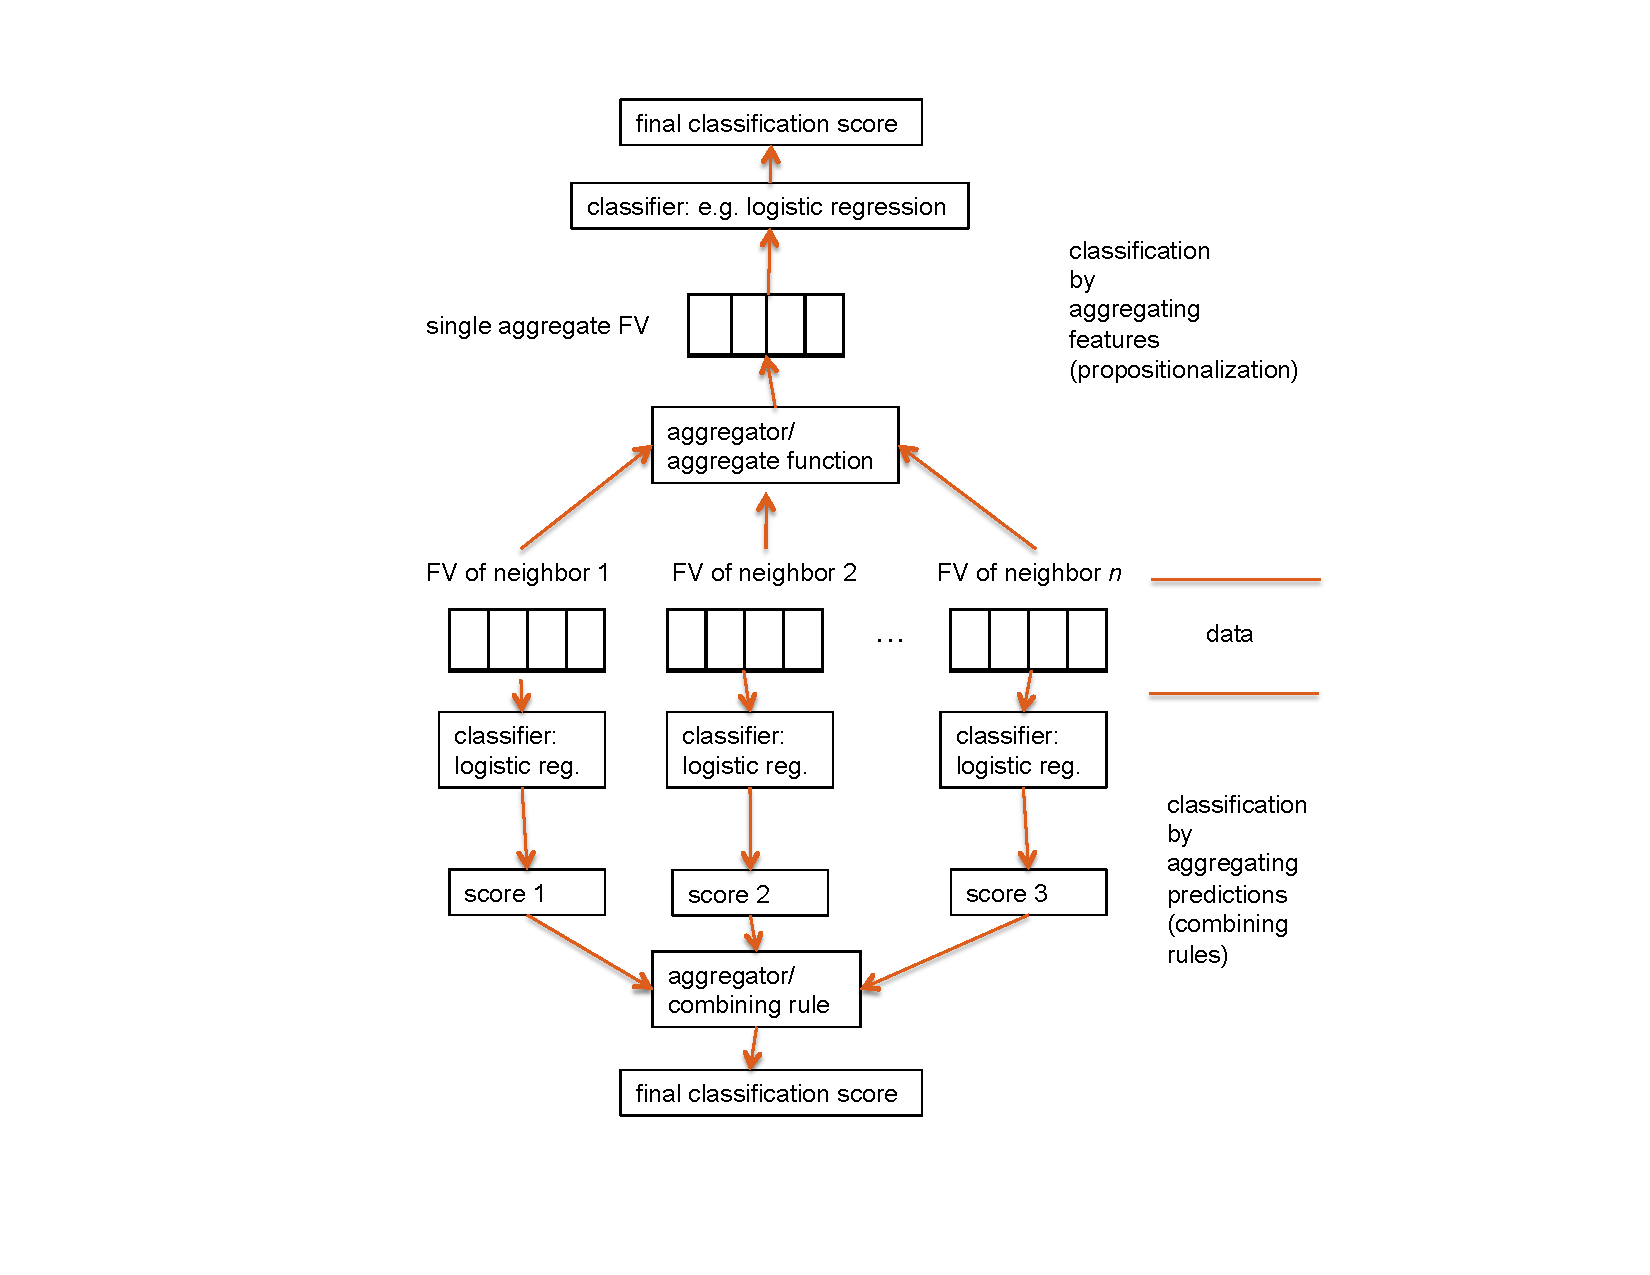
\includegraphics[width = 0.5 \textwidth]{classify}
\caption{Two different approaches to relational classification. FV = feature vector. Top: aggregating features combines the $n$ feature vectors into a single one, then applies a standard nonrelational classifier to predict a class label. Bottom: Score aggregation applies a standard nonrelational classifier to each feature vector to obtain $n$ positive class probabilities. A combining rule aggregates the $n$ scores to predict a class label.}
\label{fig:classify}
\end{center}
\end{figure}

\subsection{Aggregating Classifier Scores: Combining Rules} Most approaches that aggregate classification scores use a function that maps a list of probabilities to a single probability. Following the terminology of Bayes nets, such functions are referred to as {\em combining rules} \cite{Pearl1988,Kersting2007}. In our terminology, a combining rule is a special kind of classifier score aggregation. Our experiments examine the commonly used combining rules (e.g. average, noisy-or). Natarajan {\em et al.} \cite{Natarajan2008} review several combining rules applied with first-order logic rules.
%We use the more general concept, because some of our experiments aggregate scores that are not probabilities (e.g., the outputs of SVMs), and some aggregate probabilities but map them to a number that is not itself a probability (e.g, the geometric mean is not normalized).


\subsection{Propositionalization} The majority of work on relational classification has adopted the feature aggregation strategy.
%strategy of aggregating the features of a target entity's neighbor into a single feature vector of the target entity.
This approach of ``flattening'' the relational structure is known as {\em propositionalization} \cite{Kramer2000}. %To our knowledge, ours is the first comparison of the approach of using classifier score aggregation or combining rules vs. propositionalization.
%
For continuous features, propositionalization methods use the same standard aggregate functions as in this paper \cite{Krogel2002,C.Vens2004}.
%For discrete data, a common approach is to use a {\em feature function}. A feature function maps a relational neighborhood to a single value for the given feature. For instance, if the feature is ``student's grade is A'', the count feature function returns the number of A's achieved by the student. If the feature function returns a continuous or integer value, the values of the feature functions are used as inputs to a log-linear model (conditional random field) for prediction \cite{Sutton2007,Taskar2002,Domingos2009,Lu2003}. A feature function may also return a discrete value; a commonly used binary feature function is existential quantification, for example using 1 as a classifier if the student has achieved an A in some course, and a 0 otherwise. \marginpar{we use dummy variables}

\subsection{Learning With Aggregate Features} %The most expressive propositionalization models apply feature functions to combinations of the discrete features given in the data (e.g., \cite{Kuzelka2011}). For instance, to predict the ranking of a student, we may distinguish the number of A grades achieved in higher-level course from those achieved in lower-level courses. Complex discrete features may be combined with aggregation functions for continuous variables  \cite{C.Vens2004,Popescul2007}. For example, to predict the age of a user in a social network, we may consider the average age of her friends who have the same gender and live in the same city.

Several papers discuss advantages and disadvantages of  propositionalization for link-based classification \cite{DavidJensen2002,han2009}.
%Propositionalization has the advantages and disadvantages of general predicate invention approaches.
The main advantage is expressiveness: feature generation methods search a large space of potentially useful features. If an informative new complex feature or aggregate feature can be found, it improves classification performance and informs the user. The disadvantages are problems with both statistical and computational efficiency. Aggregation loses information in the data, which increases the variance of classifier estimates and causes problems with both type 1 and type 2 errors in feature selection \cite{DavidJensen2002}. Searching a large space of potential features presents considerable computational challenges. For an example, generating 100,000 features on the standard CiteSeer dataset, can take several CPU days (e.g., \cite[Ch.16.1.2]{Popescul2007}).

The feature aggregation method we use in this paper is intermediate between choosing a single fixed aggregate operator and searching through a space of complex expressions. For each original %unaggregated
feature, we apply a fixed set of aggregate operators (such as average, maximum, etc.). These are provided as input features to a standard learning method (e.g., logistic regression). So there is no search through a complex feature space, but learning is used to select and weight relevant aggregate features.



\subsection{Sports Statistics} The problem of predicting the results of sports matches has received considerable attention for different sports. For an overview please see \cite{Schumaker2010}. We do not claim that the methods in this paper are competitive for predicting the match results.
%For instance, the goal is usually to predict the result of a match before the game is played, so  the action counts of players in the target game are not available.
We use sports data, because they provide real-world datasets in an interesting domain with interpretable features, for the purpose of comparing aggregating features vs. aggregating predictions.

The closest predecessor to our work is that of Neville {\em et al.} \cite{Neville2003}. Key differences include the following. 1) They used only the average operator for feature aggregation, rather than a set of aggregate operators. 2)  For score aggregation, they used the arithmetic and geometric mean only. 3) They did not consider adjusting instance weights to improve score aggregation methods. 4) Their experiments used the Naive Bayes classifier applied with mainly discrete features. We use logistic regression with mainly continuous features. Continuous features are more natural for feature aggregation.

\section{Notation and Data Format} We introduce notation to discuss relational features and data and to support theoretical analysis. We follow the functor-based notation for combining statistical and relational concepts due to Poole \cite{Poole2003}.

\subsection{Functor Features}
A \textbf{population} is a set of individuals, corresponding to a domain or type in logic. A \textbf{feature} is of the form $f(t_{1},\ldots,t_{k})$ where $f$ is a functor %(either a function symbol or a predicate symbol)
 and each $t_{i}$ is a first-order variable or a constant. Each feature has a set of values (constants) called the \textbf{domain} of the feature.
%A feature whose range are the truth values $\{\true,\false\}$ is a \textbf{predicate}.
%Predicates are usually written with uppercase Roman letters, other feature with lowercase letters.
A \textbf{grounding} replaces each 1st-order variable in the feature by a constant; the result is a ground feature. A grounding may be applied simultaneously to a set of features. One of the features is the class or \textbf{target} feature. A grounding of the target feature is a \textbf{target instance}.

\subsection{Examples} In our datasets the basic populations are teams, players, matches, with corresponding first-order variables $\team, \player, \match$. Examples of features include the following.

\begin{itemize}
\item $\it{result}(\team,\match)$ denotes the result of a team in a match (win or lose). This is the target feature.
\item The ground feature $\it{result}(Canucks,1)$ denotes that the result of the Canucks in match 1. This is a target instance.
%\item $\it{PlaysFor}(\player,\team,\match)$ is a predicate that is true if player $\player$ plays for team $\team$ in match $\match$.
\item $\it{goals}(\player,\team,\match)$ is the number of goals scored by a player in a match.
\item $\plusminus(\player,\team,\match)$ is the $\plusminus$ score of a player in a match. This is a common measure of the player's performance; for precise definition see $\cite{Schumaker2010}$.
\end{itemize}

\subsection{Aggregation} Given a feature $\functor$, an aggregate function $\aggregate$ applies to one of the argument variables of $\functor$. We use the subscript notation $\aggregate_{X}$ to indicate that variable $X$ is the object of aggregation \cite{Popescul2007}. The result is a feature with one less argument. Examples include the following.

\begin{itemize}
\item $\it{goals}(\team,\match) \equiv \sum_{\player} \it{goals}(\player,\team,\match)$ is the number of goals scored by a team in a match.
\item $\it{past}\_\it{goals}(\player) \equiv \sum_{\match,\team %%\mbox{ in past season}%%
} \it{goals}(\player,\team,\match)$, where $\it{M}$ is the matches in the past season, denotes the sum of a player's goals in the past season.
%\item $\it{Past}\plusminus(\player) \equiv \sum_{\match \mbox{ in past season}} \plusminus(\player,\match)$ denotes the sum of a player's $\plusminus$ scores in the past season.
\end{itemize}

%The aggregation functions that we use in this paper are max, min, sum, midpoint, average (arithmetic mean), geometric mean.

%Suppose that we fix a \textbf{target feature} for prediction, e.g. $\it{result}(\team,\match)$. A set of features is propositionalized if only the 1st-order variables in the target feature appearing in the features in the set. For instance, $\it{goals}(\team,\match)$ is propositionalized, whereas $\it{Past}\plusminus(\player)$ is not.
%
%The simple Bayes net of Figure~\ref{fig:bn} illustrates link-based classification using the functor notation. (Bayes net with child = result, parents = plusminus(player), goals(team,match), goals(team,match,player), plays for). The random selection semantics for Bayes nets with functors views each 1st-order variable as a \cite{Schulte2013} random selection from its domain. Since a function of a random variable is also a random variable, this means that the functors in the Bayes net are also random variables. For instance, suppose that the Bayes net parameters specify the conditional probability [come up with example]. In the random selection semantics, this probability statement can be interpreted as ``[spell out]''.

\subsection{Relational Data Tables}
Relational data can be visualized in terms of the \textbf{groundings data table}. The data table has one column for each feature. It has one row for each simultaneous grounding of all functor features where the instances of the non-class features are in the neighborhood of the instance of the target feature. Thus if the target functor feature is instantiated with ground instance $\target$, the data table contains a row listing the attributes of each neighbor $\neighbor$ of $\target$. Tables~\ref{small-join} and~\ref{small-aggregate} show examples of groundings data tables. As the examples illustrate, aggregation increases the number of features (columns) and decreases the number of data points (rows). Table~\ref{small-join} is constructed as follows. A row in this table corresponds to a NHL match, one of the teams involved in the match, and one player who played for that team in the match. Each team dresses exactly 18 skaters per match, so for a given match, the data table contains $2 \times 18 = 36$ rows. The $result(\team,\match)$ column records the team result in a match, which is the target feature. The $past\_goals(\player)$ column provides a last-season statistic of the player (total number of goals). The $goals(\team,\player,\match)$ column provides a match statistic (the number of goals scored by a player in the match). The full data table used in our experiments contains 18 last-season statistics of the player %like $past\_goals(\player)$%
 and 13 match statistics 
 %like 
 %$goals(\team,\player,\match)$ 
 (see Section~\ref{sec:nhl-data}). 

\begin{table}[htbp]
\caption{Groundings Data Table for NHL.
%Features include last season aggregates  and target match statistics for players.
\label{small-join}}
\centering
\resizebox{0.5\textwidth}{!}{
\begin{tabular}{|l|l|r|l|l|r|r|}
\hline
Instance Weight & result(\team,\match) & \multicolumn{1}{l|}{MatchId \match} & TeamId \team & PlayerId \player& \multicolumn{1}{l|}{past\_goals(\player)} & \multicolumn{1}{l|}{goals(\team,\player,\match)}\\ \hline
1/18 & Loss & 2010020023 & Canucks & D. Hamhuis & 5 & 0\\ \hline
1/18 & Loss & 2010020023 & Canucks & D. Sedin & 34 & 0\\ \hline
1/18 & Loss & 2010020023 & Canucks & H. Sedin & 32 & 0\\ \hline
... & ... & %\multicolumn{1}{l|}{}
...& ...  & \#4--\#18 & ... & ... %\multicolumn{1}{l|}{}  \multicolumn{1}{l|}{} \\ \hline
\\\hline
1/18 & Win & 2010020033 & Canucks & D. Hamhuis & 5 & 0\\ \hline
1/18 & Win & 2010020033 & Canucks & C. Ehrhoff & 17 & 0\\ \hline
1/18 & Win & 2010020033 & Canucks & H. Sedin & 32 & 0\\ \hline
\end{tabular}
}
\end{table}

\begin{table}[htbp]
\caption{Aggregate Feature Data Table for NHL.
%Features are team aggregates of last season player aggregates and aggregates of player target match statistics.
}
\centering
\resizebox{0.5\textwidth}{!}{
\begin{tabular}{|l|r|l|r|r|}
\hline
result(\team,\match) & \multicolumn{1}{l|}{MatchId \match}  & TeamId \team & \multicolumn{1}{l|}{Sum\_past\_goals(\team)} & \multicolumn{1}{l|}{Sum\_goals(\team,\match)} \\ \hline
Loss & 2010020023 & Canucks & 252 & 1\\ \hline
Win & 2010020033 & Canucks & 259 & 2\\ \hline
\end{tabular}
}
\label{small-aggregate}
\end{table}


% An example of a floating figure using the graphicx package.
% Note that \label must occur AFTER (or within) \caption.
% For figures, \caption should occur after the \includegraphics.
% Note that IEEEtran v1.7 and later has special internal code that
% is designed to preserve the operation of \label within \caption
% even when the captionsoff option is in effect. However, because
% of issues like this, it may be the safest practice to put all your
% \label just after \caption rather than within \caption{}.
%
% Reminder: the "draftcls" or "draftclsnofoot", not "draft", class
% option should be used if it is desired that the figures are to be
% displayed while in draft mode.
%
%\begin{figure}[!t]
%\centering
%\includegraphics[width=2.5in]{myfigure}
% where an .eps filename suffix will be assumed under latex,
% and a .pdf suffix will be assumed for pdflatex; or what has been declared
% via \DeclareGraphicsExtensions.
%\caption{Simulation Results}
%\label{fig_sim}
%\end{figure}

% Note that IEEE typically puts floats only at the top, even when this
% results in a large percentage of a column being occupied by floats.


% An example of a double column floating figure using two subfigures.
% (The subfig.sty package must be loaded for this to work.)
% The subfigure \label commands are set within each subfloat command, the
% \label for the overall figure must come after \caption.
% \hfil must be used as a separator to get equal spacing.
% The subfigure.sty package works much the same way, except \subfigure is
% used instead of \subfloat.
%
%\begin{figure*}[!t]
%\centerline{\subfloat[Case I]\includegraphics[width=2.5in]{subfigcase1}%
%\label{fig_first_case}}
%\hfil
%\subfloat[Case II]{\includegraphics[width=2.5in]{subfigcase2}%
%\label{fig_second_case}}}
%\caption{Simulation results}
%\label{fig_sim}
%\end{figure*}
%
% Note that often IEEE papers with subfigures do not employ subfigure
% captions (using the optional argument to \subfloat), but instead will
% reference/describe all of them (a), (b), etc., within the main caption.


% An example of a floating table. Note that, for IEEE style tables, the
% \caption command should come BEFORE the table. Table text will default to
% \footnotesize as IEEE normally uses this smaller font for tables.
% The \label must come after \caption as always.
%
%\begin{table}[!t]
%% increase table row spacing, adjust to taste
%\renewcommand{\arraystretch}{1.3}
% if using array.sty, it might be a good idea to tweak the value of
% \extrarowheight as needed to properly center the text within the cells
%\caption{An Example of a Table}
%\label{table_example}
%\centering
%% Some packages, such as MDW tools, offer better commands for making tables
%% than the plain LaTeX2e tabular which is used here.
%\begin{tabular}{|c||c|}
%\hline
%One & Two\\
%\hline
%Three & Four\\
%\hline
%\end{tabular}
%\end{table}


% Note that IEEE does not put floats in the very first column - or typically
% anywhere on the first page for that matter. Also, in-text middle ("here")
% positioning is not used. Most IEEE journals/conferences use top floats
% exclusively. Note that, LaTeX2e, unlike IEEE journals/conferences, places
% footnotes above bottom floats. This can be corrected via the \fnbelowfloat
% command of the stfloats package.

%\begin{table}[htbp]
%\caption{Attribute Information Gain}
%\centering
%\resizebox{0.5\textwidth}{!}{
%\begin{tabular}{|l|l|r|l|r|l|l|r|}
%\hline
%\textbf{Dataset} & \textbf{Best Attribute} & \multicolumn{1}{l|}{\textbf{Information Gain}} & \textbf{Best Aggregated Attribute} & \multicolumn{1}{l|}{\textbf{Information %Gain}} & \textbf{STDDEV Selected?} & \textbf{STDDEV Attribute} & \multicolumn{1}{l|}{\textbf{STDDEV Information Gain}} \\ \hline
%IMDb & Director\_AvgRevenue & 0.10154 & Director\_AvgRevenue & 0.51870 & No & & \multicolumn{1}{l|}{} \\ \hline
%Financial & Remittance(Transaction) & 0.27386 & AVG(Remittance(Transaction)) & 0.35431 & Yes & STDDEV(Remittance(Transaction)) & 0.34338 \\ \hline
%NHL - Last Season and Player Match Stats & GamePlusMinus(Player) & 0.11712 & AVG(GamePlusMinus(Player)) & 0.55938 & No & & \multicolumn{1}{l|}{} \\ \hline
%NHL - Last Season Only & LastSeasonPlusMinus(Player) & 0.00138 & AVG(LastSeasonPlusMinus(Player)) & 0.00715 & Yes & STDDEV(LastSeasonShots(Player)) & 0.00342 \\ \hline
%PLG & Goals(Player) & 0.03166 & AVG(Goals(Player)) & 0.57900 & Yes & STDDEV(Goals(Player)) & 0.54300 \\ \hline
%NBA & PlusMinus(Player) & 0.17400 & AVG(PlusMinus(Player)) & 0.87400 & Yes & STDDEV(FieldGoalsMade(Player)) & 0.22800 \\ \hline
%\end{tabular}
%}
%\label{agg-information-gain}
%\end{table}


\section{Score Aggregation vs. Feature Aggregation: Strengths and Weaknesses} \label{sec:proscons} We describe carrying out relational classification with aggregate features and scores. We discuss the basic strengths and weaknesses of each approach, which motivate the design of the methods in our experiments.

Classification with aggregated features is conceptually straightforward: aggregation produces a data table with one row per target instance that can be treated like a standard attribute vector table. See Table~\ref{small-aggregate} for illustration.

Classification with aggregated scores can be visualized in terms of the \textbf{groundings data table}, or data table for short; see Table~\ref{small-join}. For simplicity, we discuss score aggregation for a single relationship, which defines a neighborhood for each grounding of the target feature. Our discussion applies equally to classification scores obtained with different types of neighborhoods.
%
Suppose that we have trained a classifier model $\classifier$ that returns a classification score for a given target label $\classlabel$ and feature vector $\features$. We write $\score_{\classifier}(\classlabel;\features)$. We can apply this classifier to each row in the groundings data table to derive a classification score from the features of each neighbor of a given target instance $\target$.
%
Given a list of classification scores, one for each row in which the target instance appears in the data table, we can apply a standard aggregation function to obtain an overall classification score. We also use the noisy-or rule for combining probabilities \cite{Kersting2007}. For a classifier whose score indicates the probability of a positive classification, such as logistic regression, we treat the aggregate probability as the overall probability of a positive classification for the target instance, as in \cite{Neville2003}.
%For other classifiers such as SVM, we classify an instance as above if the aggregate score is above the classifier's standard threshold (e.g., above 0 in the case of SVMs).
Table~\ref{table:functions-used} summarizes the aggregation functions shared by feature and score aggregation, as well as the aggregate functions specific to each method.
%When the classification scores represent probabilities, a common way to combine them is to use the ``noisy-or'' rule: [give definition]
%
%Intuitively noisy-or is a soft version of the disjunctive truth function: if any one of the probabilities is above 0.5, the combined probability is likely to be above 0.5.

\begin{table}[ht]
\caption{Aggregate Functions Used}
\centering
\resizebox{0.5\textwidth}{!}{
\begin{tabular}{|p{0.2\textwidth}|p{0.2\textwidth}|p{0.2\textwidth}|}
\hline
\multicolumn{1}{|c|}{} & \multicolumn{1}{c|}{\textbf{Feature Aggregation}} & \multicolumn{1}{c|}{\textbf{Score Aggregation}} \\ \hline
\multicolumn{ 1}{|c|}{\textbf{Shared Functions}} & \multicolumn{2}{|c|}{Average $\mu$, Maximum, Minimum, Midrange, Geometric Mean}\\ \hline
\multicolumn{ 1}{|c|}{\textbf{Specific Functions}} & Sum, Standard Deviation, Degree & Noisy--Or \\\hline
\end{tabular}
}
\label{table:functions-used}
\end{table}

\subsection{Feature Aggregation: Strengths and Weaknesses} Feature aggregation is a very common approach to relational classification and has been much discussed \cite{Neville2003,Jensen2003,han2009}. We review the main points relevant for our study. Feature aggregation is conceptually attractive as it reduces relational classification to non-relational classification with a single feature vector per target instance.  Reducing the size of the data table also speeds up learning, as our experiments show.

The obvious drawback of feature aggregation is that it loses information about the distribution of features. Consider the problem of predicting the box office receipts of a movie from user ratings. As an extreme thought experiment, suppose all movies in our dataset receive the same average user rating, but the variance of their ratings differs. Then by using the average rating as the aggregate feature, all predictive information is lost. In our experiments, we address the potential loss of information by adding a set of aggregate features to the data, rather than fixing a single aggregate operator in advance. In this way, learning can decide which aggregation operation is the most informative. Also, in addition to the mean value of a feature, we add its standard deviation as an aggregate feature. Thus learning is provided with information about the first two moments of the feature distribution rather than only the first. Adding second-moment information as an aggregate feature is discussed in \cite{Perlich2003}.

Another known problem with aggregate features is {\em degree disparity.} Degree disparity occurs when the degree, i.e., the size of a relational neighborhood, varies widely for different target instances. For example, the number of ratings received by a movie may vary from zero to thousands. One problem with using aggregate features with degree disparity is that they lose the information about the size of the relational neighborhood. Also, the values of many aggregate functions correlate with degree \cite{Jensen2003}, e.g., they tend to increase with the degree. So the aggregate feature conflates information about the degree with information about the original feature. To address this conflation, we add the relational degree of each target instance as an aggregate feature in our experiments. Adding a degree feature is recommended by \cite{Jensen2003}.

\subsection{Score Aggregation: Strengths and Weaknesses} \label{sec:score-agg} The main strength of score aggregation is that it retains the full distributional information in the data. A computational drawback is the larger data table size, which reduces speed and increases memory requirements. Another issue is applying a single fixed aggregate function to scores, rather than exploring a space of aggregate functions. A problem that figured  in our experiments, but seems not to have been previously discussed, is that score aggregation is also affected by degree disparity. As an extreme thought experiment, suppose that our dataset contains ratings for 100 movies, 99 of which have received only 1 rating, and 1 of which has received 99 ratings. So the groundings data table contains 99 rows for the one movie, and 99 rows for the other 99 movies. Hence applying a standard machine learning algorithm to the groundings data table ``as is'' overweights the movie with large degree. To address degree disparity for score aggregation, we reweight the rows in the data table by dividing by the degree of each row's target instance; see Table~\ref{small-join}. In our thought experiment, the rows for the single large-degree movie would be reweighted by 1/99, and the rows for the others would retain unit weight. Table~\ref{table:proscons} summarizes the main points of our discussion.
Our empirical evaluation examines these basic aspects of feature and score aggregation and the effectiveness of solutions to address them.

\begin{table}[htbp]
\caption{Conceptual Comparison of Feature vs. Score Aggregation}
\centering
\resizebox{0.5\textwidth}{!}{
\begin{tabular}{|c|p{0.2\textwidth}|p{0.2\textwidth}|p{0.2\textwidth}|}
\hline
\textbf{Aggregation} & \multicolumn{1}{c|}{\textbf{Pros}} & \multicolumn{1}{c|}{\textbf{Cons}} & \multicolumn{1}{c|}{\textbf{Proposed Remedy}} \\ \hline
\multicolumn{ 1}{|c|}{\textbf{Features}} & Fast learning & Loses distribution information & Utilizes multiple aggregate functions
%Add standard deviation feature 
\\
\multicolumn{ 1}{|c|}{} & Less memory required & Ignores Degree Disparity & Add degree feature\\ 
\multicolumn{ 1}{|c|}{} &  & Increases dimensionality & \\\hline
\multicolumn{ 1}{|c|}{\textbf{Scores}} & Full Distribution Information & Uses a single fixed aggregator & \\
\multicolumn{ 1}{|c|}{} &  & Degree disparity: overweights instances with many links & Reweight Instances \\\hline
\end{tabular}
}
\label{table:proscons}
\end{table}


%\begin{table}[htbp]
%\caption{Conceptual Comparison of Feature vs. Score Aggregation}
%\centering
%\resizebox{0.5\textwidth}{!}{
%\begin{tabular}{|c|p{0.2\textwidth}|p{0.2\textwidth}|}
%\hline
%\textbf{Method} & \multicolumn{1}{c|}{\textbf{Pros}} & \multicolumn{1}{c|}{\textbf{Cons}} \\ \hline
%\multicolumn{ 1}{|c|}{\textbf{Feature Aggregation}} & Fast learning & Loses distribution information \\
%\multicolumn{ 1}{|c|}{} & New feature discovery & Reduces sample size \\
%\multicolumn{ 1}{|c|}{} &  & Increases dimensionality \\ \hline
%\multicolumn{ 1}{|c|}{\textbf{Feature Aggregation+}} & As above & Increases dimensionality \\
%\multicolumn{ 1}{|c|}{} & Adds variance information &  \\ \hline
%\multicolumn{ 1}{|c|}{\textbf{Score Aggregation}} & Fixed dimensionality & Degree disparity: overweights instances with many links \\
%\multicolumn{ 1}{|c|}{} & Large sample size & Uses a single fixed aggregator \\
%\multicolumn{ 1}{|c|}{} & Full distribution information &  \\ \hline
%\multicolumn{ 1}{|c|}{\textbf{Weighted Score Aggregation}} & As above & Uses a single fixed aggregator \\
%\multicolumn{ 1}{|c|}{} & Addresses degree disparity &  \\ \hline
%\end{tabular}
%}
%\label{table:proscons}
%\end{table}


%
%
%
%\subsection{Random Selection Semantics} We can also apply the classic random selection semantics to derive a score aggregation method in a principled way \cite{Halpern90,Bacchus90}. Consider a probabilistic classifier score such as
%
%$$0.7 = P_{\classifier}(\it{result}(\team,\match) = loss; \it{past\_goals}(\player) = 10, \it{goals}(\team, \player,\match)= 2)$$
%
%On the random selection semantics, the meaning of this statement is ``if we were to randomly select a team, match, and player, there is a 0.7 probability that the class label is loss.'' With this interpretation, for a fixed target instance $\Target = \target$, the \textbf{random selection classification score}  is the expected or {\em average} score over all the neighbors of the target instance. In terms of the data table, it is the average of the scores in the rows in which the target instance appears. Therefore {\em the random selection semantics leads to using the arithmetic mean for score aggregation.}
%
%We can also use the random selection semantics for learning, not only prediction.  A common framework for learning a classifier is to tune the classifier's parameters to minimize a loss function.  For example, for probabilisic classifiers, a common loss function for a single data vector with class label $\classlabel$ and features $\features$ is the log-likelihood loss $\loss_{\classifier}(\classlabel;\features) = -\ln P_{\classifier}(\classlabel;\features)$. In terms of the data table, for a given classifier there is a loss in each row just as there is a score. Therefore the classifier's \textbf{random selection loss} on a single target instance is the average loss over the target's neighbors. The random selection loss on the entire dataset is the sum of the losses for each single target instance.
%
%In comparison, given a data matrix as input, an optimization algorithm would assess the loss for each row, then sum the losses for each row.  Without adjusting for neighborhood sizes the summation loss is biased towards target instances with larger relational neighborhoods. These observations have statistical and computational significance.
%
%(1) One of the difficulties with applying standard loss minimization to relational data is that relational datapoints are not i.i.d., but the standard summation of classifier loss over data points assume  data point independence. The random selection concept can be applied to define, in a principled way, a loss for an entire relational data table, based on a loss function for a single row.
%
%(2) Adjusting the loss function for the size of different neighborhoods requires only a small adjustment in the design of a standard classifier algorithm. If all target instances have the same number of neighbors, it is not necessary, and we can apply a standard classifier algorithm to the groundings data table.


%
%\subsection{Random Selection Classification}
%The random selection semantics suggests using the arithmetic mean for score aggregation for the following reason. On the random selection semantics, the classification scores of the classifier $\classifier$ can be interpreted as follows: For a randomly selected object $\Target$ and a randomly selected feature vector $\Features$, the classification score for $\class(\Target) = \classlabel$ given that $\Features =  \features$ is given by $\score_{\classifier}(\classlabel;\features)$. Therefore for a fixed target instance $\Target = \target$, the \textbf{random selection classification score}  neighbor is given by the expectation
%
%\begin{equation} \label{eq:exp-score}
%E[\score_{\classifier}(\classlabel)] \equiv \frac{1}{|\nbhd(\target)|} \sum_{j=1}^{|\nbhd(\target)|} \score_{\classifier}(\classlabel;\features_{j})
%\end{equation}
%where $\nbhd(\target)$ is the set of neighbors of the target instance, and $\features_{1},\ldots,\features_{|\nbhd(\target)|}$ is a list of the neighbors' features. The expression on the right hand side is the mean of the classification scores.
%
%
%\subsection{Random Selection Loss Function} A common framework for learning a classifier is to tune the classifier's parameters to minimize a loss function. One of the difficulties with applying standard loss minimization to relational data is that relational datapoints are not i.i.d., but the usual definitions of classifier loss on a dataset assume  data point independence. For example, for probabilisic classifiers, a common loss function for a single data vector with class label $\classlabel$ and features $\features$ is the log-likelihood loss $\loss_{\classifier}(\classlabel;\features) = -\ln P_{\classifier}(\classlabel;\features)$ where $P_{\classifier}(\classlabel;\features)$ denotes the probability that the classifier assigns to $\classlabel$ given as input $\features$. Given independent data rows, the class probabilities for different rows are independent of each other, and therefore the single instance loss function can be extended to the entire data table by summing the classifier losses for each row. However, relational data are not i.i.d. For example in the groundings data table, the labels of the match are the same in different rows for the same match. More generally, there are dependencies between the attributes of different entities \marginpar{cite something}
% The random selection concept can be applied to define, in a principled way, a loss for an entire relational data table, based on a loss function for a single row.  The basic idea is to use the expected loss of a classifier given a random selection of a target instance and of a neighbor. This  expected value is well-defined even for dependent data.  Formally, we define the \textbf{random selection loss} on a dataset as follows. Let $\loss_{\classifier}(\classlabel;\features)$ denote the loss of the classifier when a prediction is derived from the input features $\features$ and the true class label is $\classlabel$.
%% Given the random selection semantics, we can define the  of a classifier as the expected loss given a random selection of a target instance and of a neighbor. The formal definition is as follows.
%
%\begin{equation} \label{eq:exp-score}
%E[\loss_{\classifier}(\D)] \equiv \frac{1}{\Targetcount} \sum_{\target=1}^{\Targetcount} \frac{1}{|\nbhd(\target)|} \sum_{j=1}^{|\nbhd(\target)|}\loss_{\classifier}(\classlabel_{\target};\features_{j})
%\end{equation}
%
%where $\Targetcount$ is the number of ground instances of the target feature. In comparison, given a data matrix as input, an optimization algorithm would assess the loss for each row, then sum the losses over the rows. So given the groundings data table as input, the classification algorithm would compute the loss as
%
%\begin{equation} \label{eq:classifier-loss}
%\sum_{\target=1}^{\Targetcount} \sum_{j=1}^{|\nbhd(\target)|}\loss_{\classifier}(\classlabel_{\target};\features_{j})
%\end{equation}
%
%Comparing equations~\eqref{eq:classifier-loss} and~\eqref{eq:exp-score}, the constant $\frac{1}{\Targetcount}$ does not change the loss minima, and therefore the only relevant difference between the random selection loss and the standard summation loss is that the random selection loss scales the contribution of each target instance by the size of its neighborhood. Without such scaling the summation loss is biased towards target instances with larger relational neighborhoods. We draw the following conclusions from this analysis of the random selection semantics for classification.
%
%\begin{enumerate}
%\item  The random selection classification score for a target instance is the mean of the classification scores derived from the neighbors of the target instance.
%\item If all target instances have the same number of neighbors, we can apply a standard classifier algorithm to the groundings data table. The reason is that the standard summation loss that a classification algorithm would compute from the groundings data table is equivalent to the random selection classifier loss.
%\item If  target instances differ in the number of neighbors, the random selection loss is equivalent to averaging the losses for each target instance. This requires only a small adjustment in the design of a standard classifier algorithm.
%\end{enumerate}

% In our experiments below, the relational neighborhoods all have the same size, since the number of players per team per match is constant. Therefore the random selection semantics provides a theoretical justification for applying standard classification algorithms directly, even though there are dependencies between different rows of the data table.

\section{Datasets}
%Each method is evaluated by its ability to correctly classify the the positive class based on the features supplied. For feature aggregation, this involves aggregating the supplied features and using these aggregated features to train a SVM or Logistic Ridge Regression model and return a positive or negative classification for each instance.
%%The maximum classification accuracy of each feature aggregation model is recorded in Table~\ref{table:feture-aggregation-results}.
%
%For score aggregation, all features are first used to train a SVM or Logistic Ridge Regression model to learn a score for each row of features for a row of an instance. These scores are then grouped for each instance, and the scores are aggregated to generate an instance score and classification.
%
%The precision, negative prediction value, sensitivity, and specificity are also recorded to evaluate each model.
%
%\subsection{Hypotheses} A nice way to structure this section and to engage the referees is to give a list of what you want to establish through your experiments, before you give the details of your experiments. This usually also clarifies things for yourself. Hopefully you have more interesting hypotheses to test than ``I can find some datasets on which the predictive accuracy of my system is higher than that of some previous methods.'' The following conjecture will be evaluated:
%\begin{enumerate}
%\item Score aggregation will perform better than feature aggregation. The intuition is that aggregating features loses the information from individual player performance. By first evaluating players individually and then aggregating player scores, an improved measure of team scores can be obtained.
%\end{enumerate}
%SELF NOTE: May need to add more conjectures to this section.
%
%\subsection{Hardware and Software} The learning algorithms were executed with 64-bit Windows 7 with 12GB RAM and an Intel Core i7 2670QM CPU 2.2GHz processor. For Logistic Ridge Regression we used the L1General Matlab code \cite{bib:l1general}. For Support Vector Machine training we used the LibSVM software version 3.17 \cite{Chang2011}.
%\cite{libsvm}.

%Logistic Ridge Regression tests were completed using Java and Weka on CentOs 6.4 with 4GB RAM and an Intel Core 2 Duo CPU E6550 2.33GHz processor. Logistic Ridge Regression and SVM tests were also performed using Matlab and code from Mark Schmidt on 64-bit Windows 7 with 12GB RAM and an Intel Core i7 2670QM CPU 2.2GHz processor.

%\subsection{Datasets}

We carry out experiments on six data tables derived from five real-world databases. All our datasets are available on-line \url{http://www.sfu.ca/~kdr4/SSCI2014.zip}. The datasets vary in size and degree disparity. For each data table, we obtain two versions: the groundings data table (cf. Table~\ref{small-join}) and the feature aggregation table (cf.
Table~\ref{small-aggregate}). So each classifier is applied to twelve datasets.
Two standard databases  have been previously used in studies of relational learning, IMDb and Financial. We introduce four new datasets from three sports databases: the National Hockey League (NHL), UK Premier League (PLG), and National Basketball Association (NBA). Sports datasets are challenging for learning because of their complexity. At the same time, they are engaging to many users. They are suitable for studying the effects of aggregation because aggregate functions such as average, sum, etc. most naturally apply to continuous features, and sports datasets contain mainly continuous features, namely counts of players' actions. We describe the details of the datasets. Then we summarize the properties of the datasets that are relevant to feature and score aggregation, as discussed in Section~\ref{sec:proscons}, such as degree disparity and the variance of feature distributions.

\subsection{Dataset Details}

For each sports dataset, the target feature is $\it{result(Team,Match)}$. A positive classification means that the team is predicted to win the match. The target features for IMDb and Financial are given below.

\subsubsection{IMDb}
The hierarchical relational structure of the IMDb dataset\footnote{www.imdb.com, July 2013} is as follows: each \textit{director} has their own attributes and has directed $1$ or more \textit{movies}. Each \textit{movie} has been reviewed and rated by $1$ or more \textit{users}, who also have their own attributes. During feature aggregation, the \textit{user} attributes and ratings are aggregated. The target feature for the IMDb dataset is $\it{highBoxOffice(Movie,Director)}$, where the positive class denotes the movie had a box office receipt of $\$10,000,000$  USD or greater. The IMDb dataset contained five discrete features, which we converted to continuous 0-1 ``dummy variables'' \cite{Gelman2007}, where the presence of each discrete value is represented by a Boolean indicator variable. %The discrete features are $Gender(User)$, $Occupation(User)$,$ Genre(Movie)$, $Country(Movie)$, $ Quality(Director)$.%

\subsubsection{Financial}
The financial dataset has a hierarchical relational structure with \textit{district} at the top level, followed by \textit{accounts} within the \textit{district}, and finally all the \textit{transactions} associated with a particular \textit{account}. During feature aggregation, the attributes of the transaction are aggregated. The target feature is $\it{hasLoan(Account,District)}$, where a positive classification means there is a loan associated with the account. There were five discrete features present, which were converted to continuous ``dummy variables''. This dataset is a modified version of the financial dataset from the discovery challenge at PKDD'99 following the modification from~\cite{Yin2004}.

\subsubsection{NHL} \label{sec:nhl-data}

We used the Selenium web crawler \cite{bib:crawler} to download player game statistics (Box Scores) from \url{http://www.nhl.com/} for the seasons 2009--2013. The box scores summarize player statistics for each match, a total of 13 continuous-valued features. We refer to these as \textbf{match statistics}. We only consider skaters in our model and remove goalies, as the number of goalies in the NHL is significantly less than the number of skaters, and different statistics are recorded for goalies than skaters. The match statistics include goals, assists, plus-minus, and penalty minutes. For each player, we sum his match statistics over all NHL games in the previous season to obtain a total of 13 statistic totals for the previous season. In addition, we add 5 other season statistics: number of games played, game winning goals, power play goals, shorthanded goals, and shot percentage. We refer to the resulting 18 features as \textbf{last-season features}. From this database we prepared the following two groundings data tables, depending on whether we used last-season features only or all features.

\begin{LaTeXdescription}
\item[Season] Contains last season features only.
\item[S+Match] Contains last season features and match statistics.
%So for each match, we have 36 rows as in the Last Season dataset, and we have $19+13 = 37$ columns.
%Table~\ref{small-join} illustrates this design.
%\item[Last Season Aggregate] We apply the 6 aggregate functions max, min, sum, midpoint, average (arithmetic mean), geometric mean to each last-season feature.
%%The data table contains two rows for each match (one per team), and $1+6 \times 18 = 109$ columns.
%\item[All Features Aggregate] Same as All Features Aggregate but with aggregates of match statistics as well.
%The total number of columns is therefore $1+108+6 \times 13 = 187$ columns.
\end{LaTeXdescription}



\subsubsection{PLG}
We used Opta data~\cite{bib:opta-original}, released by Manchester City. It lists ball actions of each player in each game, for the 2011-2012 season.
%The data consists of information about the actions of a single player in a given match
%from 2011 to 2012.
Number of goals, passes and tackles by a player in a match are examples of the information associated with each player.
%Information about the teams in a season, such as number of home wins, draws or away wins can be extracted by massaging the data.
%[The information can be visualized as a heterogeneous network that links players to teams, and teams to matches. ]
For each player in a match, our data set contains 199 player actions as features.
% like $\it{TimePlayed}(\P,\M)$.
%For each team in a match, the target feature is whether the team won the match.


\subsubsection{NBA}
NBA data was obtained manually from \url{http://www.nba.com/}. Box scores containing match summary statistics for each player were used to create the data table. For each \textit{player} on a \textit{team} in a \textit{match}, there are 19 continuous player statistics recorded, such as number of free throw attempts and total number of player rebounds. These player statistics are aggregated for each $(team,match)$ instance during feature aggregation. %No team attributes or previous player statistics are used in the data table.

%\begin{table}[htbp]
%\caption{Training data for NHL Last Season and Target Match Features with Match Result}
%\begin{tabular}{|l|r|l|l|r|r|r|r|}
%\hline
%Result & \multicolumn{1}{l|}{MatchId} & TeamId & PlayerId & \multicolumn{1}{l|}{Past\_Goals(\player)} & \multicolumn{1}{l|}{Goals(\player,\team,\match)} & \multicolumn{1}{l|}{Past\_Assists(\player)} & \multicolumn{1}{l|}{Assists(\player,\team,\match)} \\ \hline
%Loss & 2010020023 & Vancouver Canucks & Dan Hamhuis & 5 & 0 & 21 & 0 \\ \hline
%Loss & 2010020023 & Vancouver Canucks & Daniel Sedin & 34 & 0 & 65 & 1 \\ \hline
%Loss & 2010020023 & Vancouver Canucks & Henrik Sedin & 32 & 0 & 94 & 1 \\ \hline
%\multicolumn{8}{c|}{\ldots} \\ \hline
%Win & 2010020033 & Vancouver Canucks & Dan Hamhuis & 5 & 0 & 21 & 0 \\ \hline
%Win & 2010020033 & Vancouver Canucks & Christian Ehrhoff & 17 & 0 & 34 & 0 \\ \hline
%Win & 2010020033 & Vancouver Canucks & Henrik Sedin & 32 & 0 & 94 & 2 \\ \hline
%\end{tabular}
%\label{small-join}
%\end{table}
%
%\begin{table}[htbp]
%\caption{Training data for NHL Last Season and Target Match Aggregated Features with Match Result}
%\begin{tabular}{|l|r|l|r|r|r|r|}
%\hline
%Result & \multicolumn{1}{l|}{MatchId} & TeamId & \multicolumn{1}{l|}{Sum\_Past\_Goals(player)} & \multicolumn{1}{l|}{Sum\_Goals(player,team,match)} & \multicolumn{1}{l|}{Avg\_Past\_Goals(player)} & \multicolumn{1}{l|}{Avg\_Goals(player,team,match)} \\ \hline
%Loss & 2010020023 & Vancouver Canucks & 252 & 1 & 14 & 0.0556 \\ \hline
%Win & 2010020033 & Vancouver Canucks & 259 & 2 & 14.3889 & 0.1111 \\ \hline
%\end{tabular}
%\label{small-aggregate}
%\end{table}
%
%Thus the random selection loss for score aggregation can be optimized by applying a standard learning algorithm to the data table as is. For the propositionalization, it is known that aggregation introduces statistical bias when the sizes of relational neighborhoods differ \cite{DavidJensen2002}, so this data set is favourable for propositionalization.


\subsection{Feature Distributions in Datasets}

We examine summary statistics for our datasets pertinent to the discussion of aggregation in Section~\ref{sec:proscons}. Table~\ref{table:rows-columns-count} shows the strong effect aggregation has on the data table dimensions. It reduces the number of rows (data points), in the case of IMDb by a factor of around 300. Aggregation increases the number of columns (features), in the case of the PLG soccer data, by a factor of almost 7.

\begin{table}[ht]
\caption{Data Table Dimensions}
\centering
\resizebox{0.5\textwidth}{!}{
\begin{tabular}{|l|r|r|r|r|}
\hline
\textbf{Dataset} & \multicolumn{1}{l|}{\textbf{Rows}} & \multicolumn{1}{l|}{\begin{tabular}{c}\textbf{Aggregated} \\ \textbf{Rows}\end{tabular}}& \multicolumn{1}{l|}{\textbf{Columns}} & \multicolumn{1}{l|}{\begin{tabular}{c}\textbf{Aggregated} \\ \textbf{Columns}\end{tabular}} \\ \hline
IMDb &  909,377  &  2,910  &  64  &  118  \\ \hline
Financial &  348,095  &  1,364  &  130  &  280  \\ \hline
NHL - S + Match  &  138,852  &  7,714  &  35  &  221  \\ \hline
NHL - Season &  138,852  &  7,714  &  22  &  130  \\ \hline
PLG &  7,933  &  580  &  203  &  1,397  \\ \hline
NBA &  767  &  60  &  23  &  137  \\ \hline
\end{tabular}
}
\label{table:rows-columns-count}
\end{table}

Table~\ref{table:variances} illustrates how aggregation decreases the variance of features. We selected one attribute for each dataset, and compared its variance on the original groundings data table to its variance after applying the average $\mu$ aggregator. A reduction in variance can be seen as a reduction in information content.

\begin{table}[ht]
\caption{Feature Variance  vs. Average Feature Variance}
\centering
\resizebox{0.5\textwidth}{!}{
\begin{tabular}{|l|l|l|l|r|}
\hline
\textbf{Dataset} & \textbf{Attribute} A & \textbf{Variance A} & \textbf{Variance $\mu$A} & \multicolumn{1}{l|}{\textbf{Reduction Ratio}} \\ \hline
IMDb & Age(User) & \multicolumn{1}{r|}{ 135.97 } & \multicolumn{1}{r|}{ 19.37 } & 7.02 \\ \hline
Financial & Amount(Transaction) & \multicolumn{1}{r|}{ 112,257,686.00 } & \multicolumn{1}{r|}{ 16,838,158.97 } & 6.67 \\ \hline
NHL - S + Match & GamePlusMinus(Player) & \multicolumn{1}{r|}{ 1.16 } & \multicolumn{1}{r|}{ 0.33 } & 3.50 \\ \hline
NHL - Season & LastSeasonPlusMinus(Player) & \multicolumn{1}{r|}{ 112.80 } & \multicolumn{1}{r|}{ 24.69 } & 4.57 \\ \hline
PLG & Goals(Player) & \multicolumn{1}{r|}{ 0.13 } & \multicolumn{1}{r|}{ 0.01 } & 13.67 \\ \hline
NBA & PlusMinus(Player) & \multicolumn{1}{r|}{ 118.02 } & \multicolumn{1}{r|}{ 38.03 } & 3.10 \\ \hline
\end{tabular}
}
\label{table:variances}
\end{table}


Table~\ref{table:degree-disparity} shows that the sports datasets have small to no degree disparity. This is because the number of players in a team in a match varies very little. In ice hockey, each NHL team dresses exactly 18 skaters per match.
% For example, in basketball, all teams dress either $12$ or $13$ players for a match.
% This is a smaller dataset than the other four datasets, and was used to examine any differences in feature and score aggregation in a small dataset as opposed to a large dataset.
The PLG dataset exhibits some small degree disparity, as a maximum of three substitutions per team are allowed during PLG matches.  The IMDb and Financial datasets exhibit considerable degree disparity, as shown in Table~\ref{table:degree-disparity}. The number of ratings for movies varies greatly. For financial transactions, different accounts may be involved in transactions to highly varying degrees of frequency.


\begin{table}[ht]
\caption{Degree Disparity}
\centering
\resizebox{0.5\textwidth}{!}{
\begin{tabular}{|l|l|r|r|r|r|}
\hline
\textbf{Dataset} & \textbf{Relationship} & \multicolumn{1}{l|}{\textbf{Average}} & \multicolumn{1}{l|}{\textbf{Standard Deviation}} & \multicolumn{1}{l|}{\textbf{Max}} & \multicolumn{1}{l|}{\textbf{Min}} \\ \hline
IMDb & Ratings/Movie &  313.91  &  411.92  &  3,427.00  &  1.00  \\ \hline
Financial & Transaction/Account &  255.68  &  134.09  &  675.00  &  9.00  \\ \hline
NHL & Players/Team,Match & 18.00 & 0.00 & 18.00 & 18.00 \\ \hline
PLG & Players/Team,Match &  13.64  &  0.63  &  14.00  &  11.00  \\ \hline
NBA & Players/Team,Match &  12.71  &  0.45  &  13.00  &  12.00  \\ \hline
\end{tabular}
}
\label{table:degree-disparity}
\end{table}

Table~\ref{agg-information-gain} examines the effect of aggregation on the apparent correlation between features and the class label. We used the information gain metric to measure the relevance of a feature to the class label. This measures the reduction in uncertainty from observing the value of the feature, 0 is the minimum and 1 the maximum value, and was computed using Weka's built-in feature selection method \cite{Hall2009}. The second column shows the attribute with the highest information gain {\em before} aggregating in the groundings data table. The last column  shows the information gain of the average $\mu$ of the best attribute in the aggregate feature table. In all cases, the information gain of the attribute increases, typically by a factor of five or more. 

There are two ways of looking at this result. Neville {\em et al.} \cite{Jensen2003,DavidJensen2002,Neville2003} argue the correlation after aggregating is overestimated, because using a single aggregate value in place of a multiset of values is like replacing each value in the multiset by the aggregate value. This underestimates the variance of the feature and overestimates its correlations to the class feature. They argue aggregation methods are liable to spurious correlations, erroneously accepting features as relevant that in fact are not. Another point of view is for features that {\em are} relevant to classification, aggregation helps to reveal the relevance. For example, in the soccer data PLG, it is intuitively clear that the number/average of goals scored by the players on a team is relevant to predicting the outcome of the match. So increasing the observed information gain is helpful for learning (see row 5 of Table~\ref{agg-information-gain}). Another example is the average revenue of a movie's director, over all of his or her movies (see row 1 of Table~\ref{agg-information-gain}). This is a feature of a movie, not of its links, and remains the same before and after aggregating movie ratings. But its information gain increases after collapsing the movie's relational neighborhood into a single vector. For datasets where aggregation highlights spurious {\em and} true correlations to the class label, an effective classifier can sort out which aggregate features are relevant for classification, and thus gain from the stronger effects. Our empirical results examine the effect of aggregation on classifier performance.

\begin{table*}[ht]
\caption{Attribute Information Gain}
\centering
\resizebox{1\textwidth}{!}{
\begin{tabular}{|l|l|r|l|r|}
\hline
\textbf{Dataset} & \textbf{Best Attribute} & \multicolumn{1}{l|}{\textbf{Information Gain}} & \textbf{$\mu$ Best Attribute} & \multicolumn{1}{l|}{\textbf{Information Gain}} \\ \hline
IMDb & Director\_AvgRevenue & 0.10154 & Director\_AvgRevenue & 0.51870 \\ \hline
Financial & Remittance(Transaction) & 0.27386 & AVG(Remittance(Transaction)) & 0.35431 \\ \hline
NHL - S + Match & PlusMinus(Player,Match) & 0.11712 & AVG$_{P}$(PlusMinus(Player,Match)) & 0.55938 \\ \hline
NHL - Season & LastSeasonPlusMinus(Player) & 0.00138 & AVG(LastSeasonPlusMinus(Player)) & 0.00715 \\ \hline
PLG & Goals(Player,Match) & 0.03166 & AVG$_{P}$(Goals(Player,Match)) & 0.57900 \\ \hline
NBA & PlusMinus(Player,Match) & 0.17400 & AVG$_{P}$(PlusMinus(Player,Match)) & 0.87400 \\ \hline
\end{tabular}
}
\label{agg-information-gain}
\end{table*}


%
%Table~\ref{table:nhl-data} provides totals for the NHL data tables.

%\begin{table}[htdp]
%\caption{Number of data points (rows) and features (columns) in the NHL data tables.}
%\begin{center}
%\begin{tabular}{c|c|c|c|c|c}
% Data Table & Last Season & All Features & Last Season Aggregate & All Features Aggregate \\ \hline
%Number Rows & 44,280 & 44,280 & 2,460 & 2,460 \\
%\hline
%Number Columns & 19 & 32 & 109 & 187
%\end{tabular}
%\end{center}
%\label{table:nhl-data}
%\end{table}%

%Table~\ref{table:nhl-data} provides summary statistics for the NHL data with player last season stats only,
%Table~\ref{table:nhl-match-data} provides summary statistics for the NHL data with player last season stats and target match statistics,
%Table~\ref{table:premier-league-data} for the Premier League data.
%
%The NHL dataset is a real-world, continuous dataset obtained using a web crawler on www.nhl.com. Player match performance and player career statistics are used as player features. The NHL dataset is also a singular dataset, as the points(player,team,match) feature is a sum of the goals(player,team,match) and assists(player,team,match) features. The Premier League dataset is a real-world, continuous dataset obtained from [GET INFORMATION] For the NHL dataset, only skaters were evaluated, and goalies were left out of the model. Each NHL team dresses exactly 18 skaters per match, which keeps a constant neighborhood size in the Bayes Net. For Premier League, the number of players on a team is variable.
%
%Models learned on the NHL dataset used the 2010-2011 matches as a training set, with 2009-2010 player statistics as the previous season statistics. Score aggregation modeling uses all 44,280 player-team-match rows for the training set. Feature aggregation uses 2,460 team-match rows.
%
%
%
%Outline the datasets that you are using. Highlight interesting aspects. Give summary statistics (e.g., data set sizes). Are they real-world or synthetic?
\section{Evaluation}

\subsection{Hardware, Methods and Comparison Metrics}
%As base classifiers, we use SVM and logistic ridge regression. For SVM, we report results for 4 kernels. Parameters of the classifiers were set by a grid search that evaluated a parameter setting by cross-validation on the training set. We report the results for the best parameter setting found by the grid search.
The learning algorithms were executed on 64-bit Windows 7 with 12GB RAM and an Intel Core i7 2670QM CPU 2.2GHz processor. As a base classifier, we use logistic ridge regression and support vector machines (SVMs). For Logistic Ridge Regression we used the L1General Matlab code \cite{bib:l1general}. For Support Vector Machine training we used the LibSVM software version 3.17 \cite{Chang2011}. Both software packages accept instance weights. Hyperparameters of the classifier were set by a grid search that evaluated a parameter setting by examining testing errors. We report the results for the best parameter setting found by the grid search.




%The methods compared are feature aggregation versus score aggregation. Feature aggregation takes all players on a team in a match, and aggregates each feature. Aggregate operators used are summation, arithmetic mean, geometric mean, maximum, minimum, and midrange. All aggregations of all features are used to train a SVM or Logistic Ridge Regression model.
%
%Score aggregation first uses player information to train a SVM or Logistic Ridge Regression model and generate player scores. These player scores are grouped for each team in a match, and the individual player scores are aggregated over each team to generate a team score.  Geometric mean was only used for Logistic Ridge Regression, as it cannot operate properly on negative values returned by a SVM model. For example, if all players on a team are assigned a negative score, the intuition would be the team is likely to lose the match. If the team has an even number of players dressed for a match, the geometric mean will return a positive score, falsely indicating the team is likely to win.


%\subsection{Performance Measures}

Our basic metrics are \textbf{classification accuracy} (percentage of correctly classified target instances) and \textbf{F1-measure}, the harmonic mean of precision and recall \cite{Witten2005}. We train the classifiers on a training set of target instances and test on the remaining target instances. All datasets use a random $80:20$ split for the training and test sets.

For feature aggregation, we report results for each dataset. All aggregations of all features are used to train the classifier. For score aggregation, we report results for pairs (Aggregate operator x Dataset). Table~\ref{table:functions-used} summarizes the aggregate operators used.
%
For score aggregation, we examine reweighting target instances by the sizes of their relational neighborhoods (see Section~\ref{sec:score-agg} and Table~\ref{small-join}). This can be easily implemented by using a classifier that accepts instance weights. We refer to datasets augmented with instance weights as x-W, as in IMDb-W and Financial-W.

\subsection{Results}

We first compare different methods for score aggregation, then for feature aggregation, finally both together. For the purpose of discussion, we refer to the average, geometric mean, and midrange operators as {\em averaging operators} since they can be viewed as a form of averaging class probabilities\footnote{midrange = ((max - min)/2)}. We refer to the remaining three maximum, minimum, and noisy-or as {\em extremal operators} since they agree with high values (maximum, noisy-or) or low values (minimum). Our main base classifier is logistic regression, so we discuss logistic regression results in most detail. We also report results for aggregating SVM scores to show that the general trends obtain with a different base classifier as well.

\subsubsection{Score Aggregation} Table~\ref{table:score-agg-lr} shows the accuracies for each combination of (logistic regression, score aggregator) for each dataset. Logistic regression provides the probability of a positive classification; aggregation functions were applied to this probability.\footnote{We also examined a more complicated method where we separately aggregated the probabilities of positive and negative classifications, then normalized the aggregates to obtain a single aggregate probability. Classification accuracy was the same.} The F1-Measures (omitted) showed the same trends as accuracy. On the datasets with substantial degree disparity (IMDb and Financial, see Table~\ref{table:degree-disparity}), scaling the importance of instances by the number of their links improved accuracy for almost all score aggregators, and led to the best overall performance. The averaging aggregators achieved good predictions on all datasets. Extremal operators can perform very well (e.g., minimum on IMDb), but also very poorly (e.g. minimum on PLG and NBA). As a default score aggregator, the average aggregator provides consistently accurate predictions. For the comparison with feature aggregation, an important observation is we do not see a dominant score aggregator across datasets. On IMDb-W, minimum is best, on Financial-W and NBA the three averaging operators, on NHL-S+Match the arithmetic average, on NHL-Season the two means, on PLG the midrange operator. These differences are statistically significant (t-test, $p<0.05$). A striking failure of the extremal operators is that for match outcome prediction, they fail to take advantage of obviously relevant match features such as the number of goals: their classification accuracy is close to using only statistics from the previous season.

Table~\ref{table:score-agg-svm} shows the result of SVMs with various kernels as a benchmark for the logistic regression results. For a single input feature vector, SVMs produce an output score, to which we apply aggregate functions. We experienced problems with numeric instability in computing the geometric mean of SVM scores, so we do not report the results for SVM score aggregation with the geometric mean. The results for score aggregation with SVMs depend on the kernel used. The best performance over all results was achieved with the linear kernel. These results are slightly worse than with logistic regression, except for the IMDb and Financial datasets. On the first five datasets, score aggregation with the Gaussian kernel tends to assign all test instances as positive, and produces the random classification accuracy of 50\%. The quadratic kernel leads to 50\% accuracy on all eight datasets, so we do not list these results.
We observe the same trends as with logistic regression: There is considerable variability among the classification accuracy of different score aggregation functions. Averaging operators produce reliable baseline performance.

The variability in predictive accuracy suggests that finding a good score aggregation method requires experimentation and/or a learning method. Methods for learning a good score aggregation method for a given dataset are an interesting topic for future work. In contrast, standard feature selection techniques can be used to select a good feature aggregator for a dataset, as our next set of experiments show.%In the next experiments we examine the performance of our straightforward approach where the original feature space is expanded with a fixed set of aggregated features.


%Weighting the rows of IMDb and Financial groundings data tables with the degrees of each instance slightly improved the best classification accuracy. %SVMs performed poorly overall, with the exceptions of using the linear or quadratic kernel with the average score aggregator. Logistic regression is superior to SVMs when used with score aggregation on these datasets.
%The average operator worked best for Linear and Quadratic SVMs.

\begin{table*}[ht]
\caption{Score Aggregation Accuracies - Logistic Regression}
\centering
\resizebox{1\textwidth}{!}{
\begin{tabular}{|l|r|r|r|r|r|r|r|r|}
\hline
\textbf{Aggregator} & \multicolumn{1}{l|}{IMDb} & \multicolumn{1}{l|}{IMDb-W} &\multicolumn{1}{l|}{Financial} & \multicolumn{1}{l|}{Financial-W} &\multicolumn{1}{l|}{NHL - S + Match} & \multicolumn{1}{l|}{NHL - Season} & \multicolumn{1}{l|}{PLG} & \multicolumn{1}{l|}{NBA} \\ \hline
Average & 78.52\% & 81.44\% & 69.12\% & 73.16\% & \textbf{87.29\%} & \textbf{55.25\%} & 90.52\% & \textbf{100.00\%} \\ \hline
Geometric Mean & 78.69\% & 81.44\% & 69.49\% & 72.43\% & 85.08\% & 55.12\% & 81.03\% & \textbf{100.00\%} \\ \hline
Midrange & 78.52\% & 80.93\% & \textbf{72.79\%} & \textbf{73.53\%} & 85.34\% & 52.79\% & \textbf{93.10\%} & \textbf{100.00\%} \\ \hline
Maximum & 71.65\% & \textbf{82.13\%} & 63.97\% & 68.75\% & 52.01\% & 50.65\% & 53.45\% & 50.00\% \\ \hline
Noisy-Or & 71.65\% & \textbf{82.13\%} & 63.97\% & 64.34\% & 52.01\% & 50.65\% & 53.45\% & 50.00\% \\ \hline
Minimum & \textbf{81.79\%} & 79.73\% & 53.68\% & 51.10\% & 50.45\% & 50.00\% & 51.72\% & 58.33\% \\ \hline
\end{tabular}
}
\label{table:score-agg-lr}
\end{table*}

\begin{table*}[ht]
\caption{Score Aggregation Accuracies - Support Vector Machines}
\centering
\resizebox{1\textwidth}{!}{
\begin{tabular}{|l|l|r|r|r|r|r|r|r|r|}
\hline
\textbf{Kernel Type} & \textbf{Aggregator} & \multicolumn{1}{l|}{IMDb} & \multicolumn{1}{l|}{IMDb-W} &\multicolumn{1}{l|}{Financial} & \multicolumn{1}{l|}{Financial-W} &\multicolumn{1}{l|}{NHL - S + Match} & \multicolumn{1}{l|}{NHL - Season} & \multicolumn{1}{l|}{PLG} & \multicolumn{1}{l|}{NBA} \\ \hline
\multicolumn{1}{|l|}{Linear} & Average & \textbf{82.30\%} & 50.00\% & 74.63\% & \textbf{71.69\%} & 73.61\% & 53.05\% & 90.52\% & \textbf{100.00\%} \\ \cline{2-10}
\multicolumn{1}{|l|}{} & Midrange & \textbf{82.30\%} & 50.00\% & \textbf{75.00\%} & 62.87\% & \textbf{74.38\%} & 51.49\% & \textbf{92.24\%} & \textbf{100.00\%} \\ \cline{2-10}
\multicolumn{1}{|l|}{} & Maximum & \textbf{82.30\%} & 50.00\% & 62.87\% & 62.87\% & 59.73\% & 51.82\% & 59.48\% & 50.00\% \\ \cline{2-10}
\multicolumn{1}{|l|}{} & Minimum & \textbf{82.30\%} & 50.00\% & 54.78\% & 50.00\% & 57.00\% & 51.75\% & 50.86\% & 58.33\% \\ \hline
%\multicolumn{1}{|l|}{Quadratic} & Average &  &  & 50.00\% &  & 50.00\% & 50.00\% & 50.00\% & 50.00\% \\ \cline{2-10}
%\multicolumn{1}{|l|}{} & Midrange &  &  & 50.00\% &  & 50.00\% & 50.00\% & 50.00\% & 50.00\% \\ \cline{2-10}
%\multicolumn{1}{|l|}{} & Maximum &  &  & 50.00\% &  & 50.00\% & 50.00\% & 50.00\% & 50.00\% \\ \cline{2-10}
%\multicolumn{1}{|l|}{} & Minimum &  &  & 50.00\% &   & 50.00\% & 50.00\% & 50.00\% & 50.00\% \\ \hline
\multicolumn{1}{|l|}{Gaussian} & Average & 50.00\% & 50.00\% & 50.00\% & 50.00\% & 50.00\% & \textbf{53.44\%} & 73.28\% & \textbf{100.00\%} \\ \cline{2-10}
\multicolumn{1}{|l|}{} & Midrange & 50.00\% & 50.00\% & 50.00\% & 50.00\% & 50.00\% & 51.62\% & 71.55\% & \textbf{100.00\%} \\ \cline{2-10}
\multicolumn{1}{|l|}{} & Maximum & 50.00\% & 50.00\% & 50.00\% & 50.00\% & 50.00\% & 53.11\% & 61.21\% & 50.00\% \\ \cline{2-10}
\multicolumn{1}{|l|}{} & Minimum & 50.00\% & 50.00\% & 50.00\% & 50.00\% & 50.00\% & 50.00\% & 50.00\% & 58.33\% \\ \hline
\end{tabular}
}
\label{table:score-agg-svm}
\end{table*}

%\begin{table}[htbp]
%\caption{NHL Results. Logistic Regression is  used both with the predicted probability (Prob) and the log-probability (Log-Prob). The random selection classifier uses Average %+ Log-Prob. Italics indicate the best SVM classifier.}
%\begin{subtable}[htbp]
%\centering
%\resizebox{0.5\textwidth}{!}{
%\caption{Last Season Statistics Only}
%\begin{tabular}{|l|r|r|r|r|r|}
%\hline
% Last Season & \multicolumn{4}{c|}{Score Aggregator} \\ \hline
% & \multicolumn{ 1}{c|}{Average} & \multicolumn{ 1}{c|}{Maximum} & \multicolumn{ 1}{c|}{Minimum} &
%\multicolumn{ 1}{c|}{Noisy-Or} \\\hline \cline{ 1- 1}
%SVM - Linear & \textit{53.59\%} & 50.57\% & \textbf{50.45\%} & 50.57\% \\ \hline
%SVM - Quadratic & 50.89\% & 50.00\% & 50.00\% & \textbf{50.69\%} \\ \hline
%SVM - Sigmoid & 50.00\% & 50.00\% & 50.00\%  & 50.00\% \\ \hline
%SVM - Gaussian & 50.00\% & 50.00\% & 50.00\% & 50.00\% \\ \hline
%LR - Prob & \textbf{54.43\%} & \textbf{54.43\%} & 50.42\% & 50.00\% \\ \hline
%LR - Log-Prob & 54.39\% & \textbf{54.43\%} & 50.42\% & N/A \\ \hline
%\end{tabular}
%}
%\label{default}
%\end{subtable}%

%\begin{subtable}[htbp]
%\centering
%\resizebox{0.5\textwidth}{!}{
%\subcaption{Last S + Match Features}
%\begin{tabular}{|l|r|r|r|r|r|}
%\hline
% All Features & \multicolumn{4}{c|}{Score Aggregator}\\ \hline
% & \multicolumn{ 1}{c|}{Average} & \multicolumn{ 1}{c|}{Maximum} & \multicolumn{ 1}{c|}{Minimum} &
%\multicolumn{ 1}{c|}{Noisy-Or}  \\\hline \cline{ 1- 1}
%SVM - Linear & 73.46\% & 50.73\% & \textbf{57.51\%} & \textbf{52.82\%} \\ \hline
%SVM - Quadratic & \textit{80.91\%} & 53.78\% & 53.92\% & 51.87\% \\ \hline
%SVM - Sigmoid & 50.00\% & 50.00\% & 50.00\% & 50.00\% \\ \hline
%SVM - Gaussian & 50.00\% & 50.00\% & 50.00\% & 50.00\% \\ \hline
%LR - Prob & \textbf{87.26\%} & \textbf{87.26\%} & 54.89\% & 51.67\% \\ \hline
%LR - Log-Prob & 86.60\% & \textbf{87.26\%} & 54.89\% & N/A \\ \hline
%\end{tabular}
%}
%\label{table:nhl-score}
%\end{subtable}%
%\end{table}%

\subsubsection{Feature Aggregation}

Table~\ref{table:feat-agg-lr-acc} presents the results for logistic regression applied with feature aggregation methods, on all six datasets. The F1-Measures (omitted) showed the same trends as accuracy. Adding the standard deviation of continuous features tended to improve predictions, but only the difference on Financial was statistically significant. 
%There is clearly improvement potential for a more sophisticated way of using variance information. 
Examination of regression weights showed average and sum of plus-minus and goals to be strong predictors for sports datasets.

%Since feature aggregation produces a standard data table, we can apply any classifier, including nonprobabilistic ones, to benchmark logistic regression.
Table~\ref{table:feat-agg-svm-acc} shows the result of SVMs with various kernels (including the standard deviation aggregate feature). Comparing with Table~\ref{table:feat-agg-lr-acc}, we see that logistic regression performs well on the aggregated datasets compared to SVMs. Also, among the SVM kernels, the linear kernel provides accurate predictions. Together with the success of logistic regression, these results indicate that aggregation makes our datasets close to linearly separable. This is another way in which feature aggregation can improve classification, despite the loss of information it entails.

%Experiments were also performed using SVMs, results shown in Table~\ref{table:feat-agg-svm-acc}.
%Adding the standard deviation as an aggregate feature only made significant improvements to the Financial dataset.

\begin{table*}[ht]
\caption{Feature Aggregation Accuracies - Logistic Regression}
\centering
\resizebox{1\textwidth}{!}{
\begin{tabular}{|l|r|r|r|r|r|r|}
\hline
\textbf{Method} & \multicolumn{1}{l|}{IMDb} &\multicolumn{1}{l|}{Financial} &\multicolumn{1}{l|}{NHL - S + Match} & \multicolumn{1}{l|}{NHL - Season} & \multicolumn{1}{l|}{PLG} & \multicolumn{1}{l|}{NBA} \\ \hline
Logistic Regression & \textbf{86.05\%} & 84.93\% & 88.59\% & \textbf{54.67\%} & 95.69\% & \textbf{100.00\%} \\ \hline
Logistic Regression & 85.57\% & \textbf{87.50\%} & \textbf{88.91\%} & 54.47\% & \textbf{96.55\%} & \textbf{100.00\%} \\
+ standard deviation   &&&&&&\\
\hline
\end{tabular}
}
\label{table:feat-agg-lr-acc}
\end{table*}

\begin{table*}[ht]
\caption{Feature Aggregation Accuracies - Support Vector Machines}
\centering
\resizebox{1\textwidth}{!}{
\begin{tabular}{|l|r|r|r|r|r|r|}
\hline
\textbf{Method} & \multicolumn{1}{l|}{IMDb} &\multicolumn{1}{l|}{Financial} &\multicolumn{1}{l|}{NHL - S + Match} & \multicolumn{1}{l|}{NHL - Season} & \multicolumn{1}{l|}{PLG} & \multicolumn{1}{l|}{NBA} \\ \hline
SVM - Linear & \textbf{84.54\%} & \textbf{76.84\%} & 68.03\% & \textbf{55.12\%} & \textbf{95.69\%} & \textbf{100.00\%}\\ \hline
%SVM - Linear & 81.79\% & \textbf{76.84\%} & 68.03\% & \textbf{55.12\%} & 95.69\% & \textbf{100.00\%}\\ \hline
%SVM - Linear + $\sigma$ & \textbf{84.54\%} & 74.63\% & 66.15\% & 53.83\% & 95.69\% & \textbf{100.00\%} \\ \hline
SVM - Quadratic & 71.99\% & 72.06\% & \textbf{68.94\%} & 52.66\% & 90.52\% & 91.67\%\\ \hline
%SVM - Quadratic & 71.99\% & 72.06\% & 61.74\% & 52.66\% & 89.71\% & 91.67\%\\ \hline
%SVM - Quadratic + $\sigma$ & 71.99\% & 72.06\% & \textbf{68.94\%} & 53.76\% & 90.52\% & 83.33\% \\ \hline
SVM - Gaussian & 82.30\% & 65.81\% & 60.38\% & 52.75\% & 87.93\%  & \textbf{100.00\%} \\ \hline
%SVM - Gaussian & 82.30\% & 65.81\% & 52.52\% & 50.00\% & 54.78\% & \textbf{100.00\%} \\ \hline
%SVM - Gaussian + $\sigma$ & 82.30\% & 65.81\% & 60.38\% & 52.75\% & 87.93\% & \\ \hline
\end{tabular}
}
\label{table:feat-agg-svm-acc}
\end{table*}

\begin{table*}[ht]
\caption{Feature Aggregation vs. Score Aggregation}
\centering
\resizebox{1\textwidth}{!}{
\begin{tabular}{|l|r|r|r|r|r|r|r|r|r|r|r|r|}
\hline
Dataset $\rightarrow$ & \multicolumn{2}{|c|}{IMDb} & \multicolumn{2}{c|}{Financial} & \multicolumn{2}{c|}{NHL - S + Match} & \multicolumn{2}{c|}{NHL - Season} & \multicolumn{2}{c|}{PLG} & \multicolumn{2}{c|}{NBA} \\ \hline
Method $\downarrow$& \multicolumn{1}{l|}{Accuracy} & \multicolumn{1}{l|}{F1-Measure} & \multicolumn{1}{l|}{Accuracy} & \multicolumn{1}{l|}{F1-Measure} & \multicolumn{1}{l|}{Accuracy} & \multicolumn{1}{l|}{F1-Measure} & \multicolumn{1}{l|}{Accuracy} & \multicolumn{1}{l|}{F1-Measure} & \multicolumn{1}{l|}{Accuracy} & \multicolumn{1}{l|}{F1-Measure} & \multicolumn{1}{l|}{Accuracy} & \multicolumn{1}{l|}{F1-Measure} \\ \hline
Feature Aggregation & \textbf{86.05\%} & \textbf{0.86} & \textbf{87.50\%} & \textbf{0.87} & \textbf{88.91\%} & \textbf{0.89} & 55.12\% & \textbf{0.59} & \textbf{96.55\%} & \textbf{0.96} & \textbf{100.00\%} & \textbf{1.00} \\ \hline
Score Aggregation & 82.30\% & 0.85 & 75.00\% & 0.78 & 87.35\% & 0.87 & \textbf{55.25\%} & 0.46 & 93.10\% & 0.93 & \textbf{100.00\%} & \textbf{1.00} \\ \hline
\end{tabular}
}
\label{table:summary-results}
\end{table*}


%\begin{table*}[htbp]
%\caption{Detailed Feature Aggregation vs. Score Aggregation}
%\centering
%\resizebox{1\textwidth}{!}{
%\begin{tabular}{|l|r|r|r|r|r|r|r|r|r|r|r|r|}
%\hline
%Dataset $\rightarrow$& \multicolumn{ 2}{c|}{IMDb} & \multicolumn{ 2}{c|}{Financial} & \multicolumn{ 2}{c|}{NHL - S + Match} & \multicolumn{ 2}{c|}{NHL - Season} & \multicolumn{ 2}{c|}{PLG} & \multicolumn{ 2}{c|}{NBA} \\ \hline
%Method $\downarrow$& \multicolumn{1}{l|}{Accuracy} & \multicolumn{1}{l|}{F1-Measure} & \multicolumn{1}{l|}{Accuracy} & \multicolumn{1}{l|}{F1-Measure} & \multicolumn{1}{l|}{Accuracy} & \multicolumn{1}{l|}{F1-Measure} & \multicolumn{1}{l|}{Accuracy} & \multicolumn{1}{l|}{F1-Measure} & \multicolumn{1}{l|}{Accuracy} & \multicolumn{1}{l|}{F1-Measure} & \multicolumn{1}{l|}{Accuracy} & \multicolumn{1}{l|}{F1-Measure} \\ \hline
%Feature Agg. & \textbf{86.05\%} & \textbf{0.86} & 84.93\% & 0.84 & 88.59\% & \textbf{0.89} & 54.67\% & 0.49 & 95.69\% & \textbf{0.96} & \textbf{100.00\%} & \textbf{1.00} \\ \hline
%Feature Agg. + $\sigma$ & 85.57\% & \textbf{0.86} & \textbf{87.50\%} & \textbf{0.87} & \textbf{88.91\%} & \textbf{0.89} & 54.47\% & \textbf{0.50} & \textbf{96.55\%} & \textbf{0.96} & \textbf{100.00\%} & \textbf{1.00} \\ \hline
%Score Agg. - Best & \multicolumn{1}{l|}{81.79\% (Min)} & 0.84 & \multicolumn{1}{l|}{72.79\% (Mid)} & 0.77 & \multicolumn{1}{l|}{87.29\% (Avg)} & 0.87 & \multicolumn{1}{l|}{\textbf{55.25\% (Avg)}} & 0.46 & \multicolumn{1}{l|}{93.10\% (Mid)} & 0.93 & \multicolumn{1}{l|}{\textbf{100.00\% (Avg)}} & \textbf{1.00} \\ \hline
%Score Agg. - $\mu$ & 78.52\% & 0.82 & 69.12\% & 0.74 & 87.29\% & 0.87 & \textbf{55.25\%} & 0.46 & 90.52\% & 0.90 & \textbf{100.00\%} & \textbf{1.00} \\ \hline
%Weighted S.Agg. - Best & \multicolumn{1}{l|}{82.13\% (Max)} & 0.82 & \multicolumn{1}{l|}{73.53\% (Mid)} & 0.76 & \multicolumn{1}{l|}{87.35\% (Avg)} & 0.87 & \multicolumn{1}{l|}{55.12\% (Avg)} & 0.48 & \multicolumn{1}{l|}{92.24\% (Mid)} & 0.92 & \multicolumn{1}{l|}{\textbf{100.00\% (Avg)}} & \textbf{1.00} \\ \hline
%Weighted S. Agg. - $\mu$ & 81.44\% & 0.81 & 73.16\% & 0.74 & 87.35\% & 0.87 & 55.12\% & 0.48 & 90.52\% & 0.90 & \textbf{100.00\%} & \textbf{1.00} \\ \hline
%\end{tabular}
%}
%\label{table:lr-results}
%\end{table*}


\begin{table*}[ht]
\caption{Learning Time in Seconds}
\centering
\resizebox{1\textwidth}{!}{
\begin{tabular}{|l|r|r|r|r|r|r|}
\hline
\multicolumn{ 1}{|c|}{} & \multicolumn{ 1}{c|}{IMDb} & \multicolumn{ 1}{c|}{Financial} & \multicolumn{ 1}{c|}{NHL - S + Match} & \multicolumn{ 1}{c|}{NHL - Season} & \multicolumn{ 1}{c|}{PLG} & \multicolumn{ 1}{c|}{NBA} \\ \hline
Feature Aggregation & 0.083 & 0.894 & 0.523 & 0.126 & 3.288 & 0.034 \\ \hline
Score Aggregation & 14.074 & 6.314 & 0.567 & 0.229 &0.430 & 0.004 \\ \hline
\end{tabular}
}
\label{learning-times}
\end{table*}

\subsubsection{Score Aggregation vs. Feature Aggregation} Table~\ref{table:summary-results} compares the best feature aggregation method with the best score aggregation method, for the logistic regression base classifier.
Feature aggregation has statistically significant greater classification accuracy and F1-measure than score aggregation on all datasets, with the exception of the NHL-Season and NBA datasets, where there is no statistically significant difference. On the Financial dataset, feature aggregation outperforms score aggregation by a wide margin of $12.50\%$.
Feature aggregation outperforms score aggregation the most on the two datasets with the greatest degree disparity. Together with the results of Table~\ref{table:score-agg-lr}, this is evidence that degree disparity causes problems for score aggregation as well as feature aggregation.

Table~\ref{learning-times} shows that aggregation can speed up learning considerably by reducing the number of data points (e.g., speed up factor of 15 on IMDb). The trade-off is the number of extra features added, which can slow down aggregation, as we observe on the PLG soccer data set.
%
%In sum, comparing score aggregators, the arithmetic and geometric mean appears to be the most robust aggregator, providing competitive performance in a variety of settings. %The noisy-or operator performed poorly on all datasets.

%In tests for both aggregation methods, F1-Measure correlated closely with classification accuracy.

%Comparing feature aggregators, there was no single operator that %%Minimum and noisy-or aggregate operators demonstrated poor performance on all datasets.
%When using the maximum aggregate operator, logistic ridge regression showed a strong improvement in classification accuracy over SVMs.

%The fact that sometimes feature aggregation outperforms score agggregations suggests that there aggregated features can benefit classification.


\section{Conclusion}


We considered relational classification with continuous features of linked entities. Two basic approaches are aggregating features vs. aggregating classifier scores. For aggregating classifier scores using a combining rule, averaging-type rules provide consistent good baseline performance. On some datasets, they can be outperformed by extremal rules, such as maximum or noisy-or.

For feature aggregation, we investigated an approach to finding relevant aggregate features by applying a fixed set of aggregate operators to each original feature, then applying a standard classifier to the aggregate features. This use of feature aggregation outperforms score aggregation, even when matched against the best score aggregation rule selected a posteriori. While feature aggregation has well-known statistical problems, part of the reason for its superior performance is that score aggregation suffers from similar challenges. For instance, degree disparity is a challenge for both approaches, because in score aggregation, target instances with more links carry more weight than those with fewer.

{\em Future Work.} An open challenge for score aggregation is whether a good combining rule can be learned for a specific dataset. This question seems to be quite open.
Jaeger \cite{Jaeger2007} proposes learning linear combinations of combining rules for relational Bayesian networks; it may be possible to adapt this approach for large-scale
relational classification.

A hybrid approach that combines score aggregation with feature aggregation could address the weaknesses of both approaches.
For example good features could be found learning a model based on feature aggregation. Adding  good aggregation features to non-aggregated features (e.g., adding team aggregate statistics to individual player statistics) could then improve classification accuracy in score aggregation.

In sum, good accuracy in relational classification can be achieved with both feature aggregation and score aggregation (when used with averaging-type aggregators). We found that standard feature weighting techniques for selecting among aggregate features led to consistently superior classification performance.


% conference papers do not normally have an appendix


% use section* for acknowledgement
%\section*{Acknowledgment}


%The authors would like to thank...





% trigger a \newpage just before the given reference
% number - used to balance the columns on the last page
% adjust value as needed - may need to be readjusted if
% the document is modified later
%\IEEEtriggeratref{8}
% The "triggered" command can be changed if desired:
%\IEEEtriggercmd{\enlargethispage{-5in}}

% references section

% can use a bibliography generated by BibTeX as a .bbl file
% BibTeX documentation can be easily obtained at:
% http://www.ctan.org/tex-archive/biblio/bibtex/contrib/doc/
% The IEEEtran BibTeX style support page is at:
% http://www.michaelshell.org/tex/ieeetran/bibtex/
%\bibliographystyle{IEEEtran}
% argument is your BibTeX string definitions and bibliography database(s)
%\bibliography{IEEEabrv,../bib/paper}
%
% <OR> manually copy in the resultant .bbl file
% set second argument of \begin to the number of references
% (used to reserve space for the reference number labels box)
\bibliographystyle{IEEEtran}
\bibliography{master}




% that's all folks
\end{document}


